\title{CS313 : DataBases and Information Systems Lab \\
    \vspace{0.6cm}
    Lab Assignment 4
} % You may change the title if you want.
% \subtitle{Hello}
\author{Sourabh Bhosale \\ 200010004}

\date{\today}

\documentclass[12pt]{article}
\usepackage{fullpage}
\usepackage{enumitem}
\usepackage{amsmath,mathtools}
\usepackage{amssymb}
\usepackage[super]{nth}
\usepackage{textcomp}
\usepackage{hyperref}
\usepackage{multicol}
\usepackage{multirow}
\usepackage{minted}
% \usepackage{fontspec}
% \usepackage[showframe]{geometry}

% \usepackage[default]{sourcesanspro}
% \usepackage[T1]{fontenc}

% \usepackage[sfdefault]{noto}
% \usepackage[T1]{fontenc}

\usepackage[default,oldstyle,scale=0.95]{opensans} %% Alternatively
%% use the option 'defaultsans' instead of 'default' to replace the
%% sans serif font only.
\usepackage[T1]{fontenc}

% \setmainfont{Roboto}
\usepackage{titling}
\hypersetup{
    colorlinks=true,
    linkcolor=blue,
    filecolor=magenta,      
    urlcolor=cyan,
}

\renewcommand\maketitlehooka{\null\mbox{}\vfill}
\renewcommand\maketitlehookd{\vfill\null}

\begin{document}


\begin{titlingpage}
\maketitle
\end{titlingpage}

\newpage
%---------------------------------------------------------------------

\section{Creating user called universityDB0004}

\subsection{Query}
\fbox{ 
    \begin{minipage}{40em}
    \inputminted{mysql}{src/1.sql}
    \end{minipage}
}

\subsection{Result}
\begin{figure}[!hbt]
    \centering
    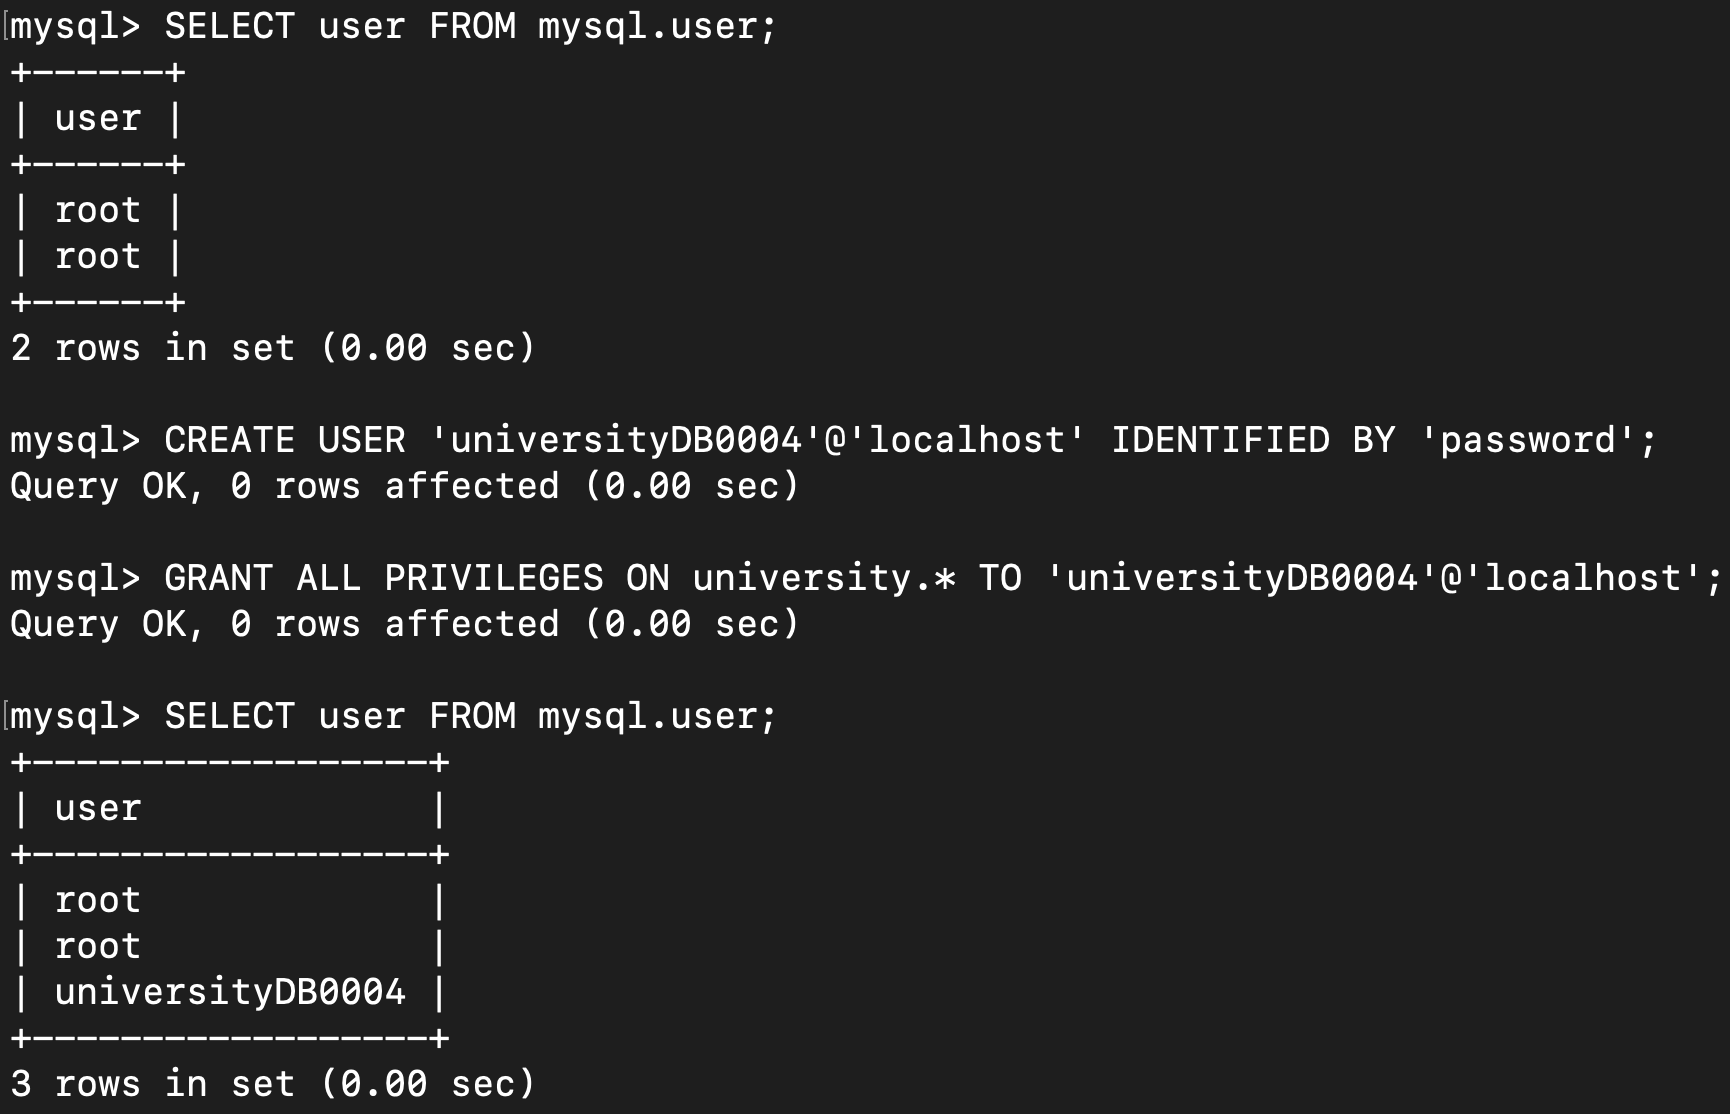
\includegraphics[scale=0.6]{screenshots/1.png}
    \label{fig:my_label1}
\end{figure}

\newpage
%---------------------------------------------------------------------

\section{Creating database called university}

\subsection{Query}
\fbox{ 
    \begin{minipage}{40em}
    \inputminted{mysql}{src/2.sql}
    \end{minipage}
}

\subsection{Result}
\begin{figure}[!hbt]
    \centering
    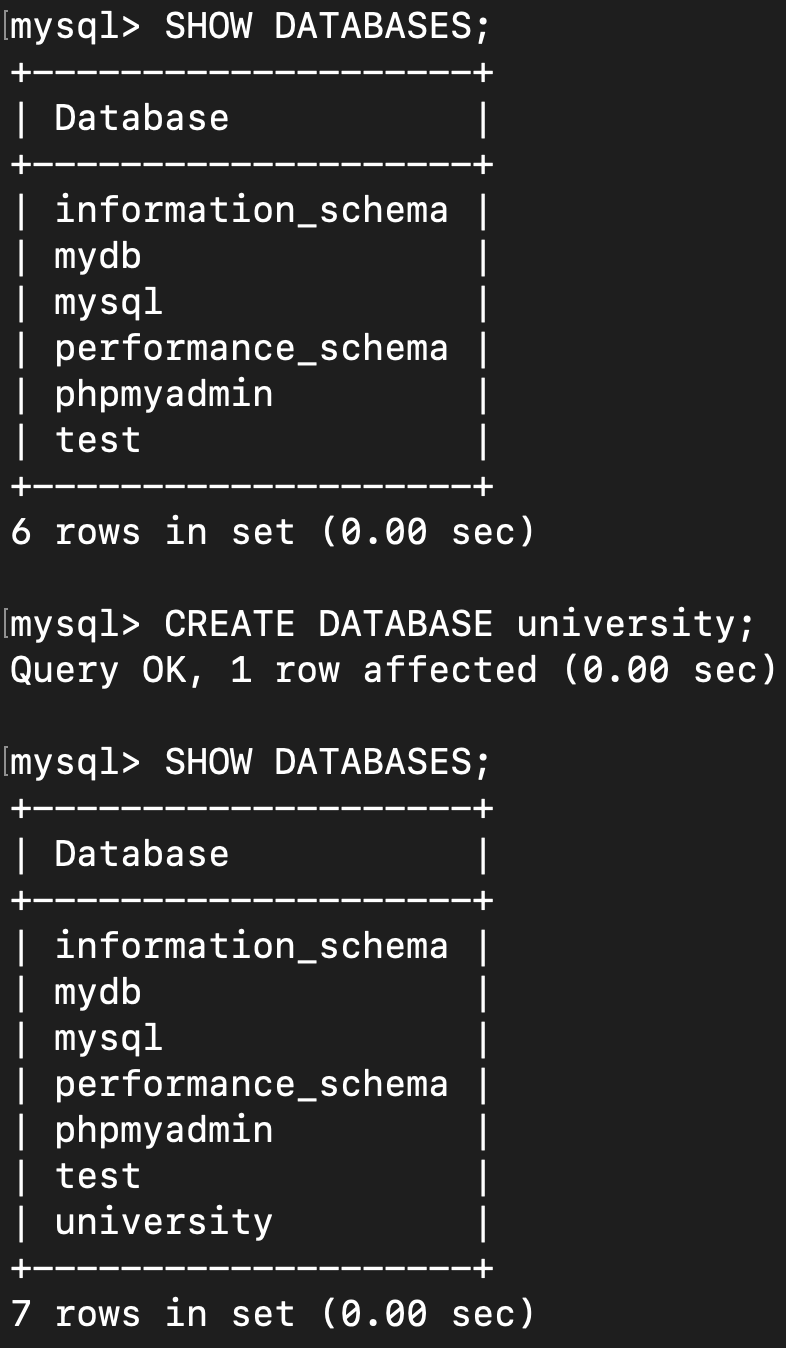
\includegraphics[scale=0.7]{screenshots/2.png}
    \label{fig:my_label1}
\end{figure}

\newpage
%---------------------------------------------------------------------
\section{Connecting to database called university}

\subsection{Query}
\fbox{ 
    \begin{minipage}{40em}
    \inputminted{mysql}{src/3.sql}
    \end{minipage}
}

\subsection{Result}
\begin{figure}[!hbt]
    \centering
    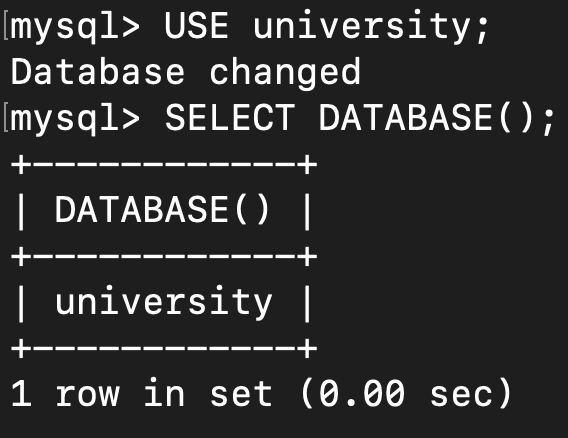
\includegraphics[scale=1.7]{screenshots/3.png}
    \label{fig:my_label1}
\end{figure}

\newpage
%---------------------------------------------------------------------

\section{Creating tables in the database using DDL.sql file}

\subsection{Query}
\fbox{ 
    \begin{minipage}{40em}
    \inputminted{mysql}{src/4.sql}
    \end{minipage}
}

\subsection{Result}
\begin{figure}[!hbt]
    \centering
    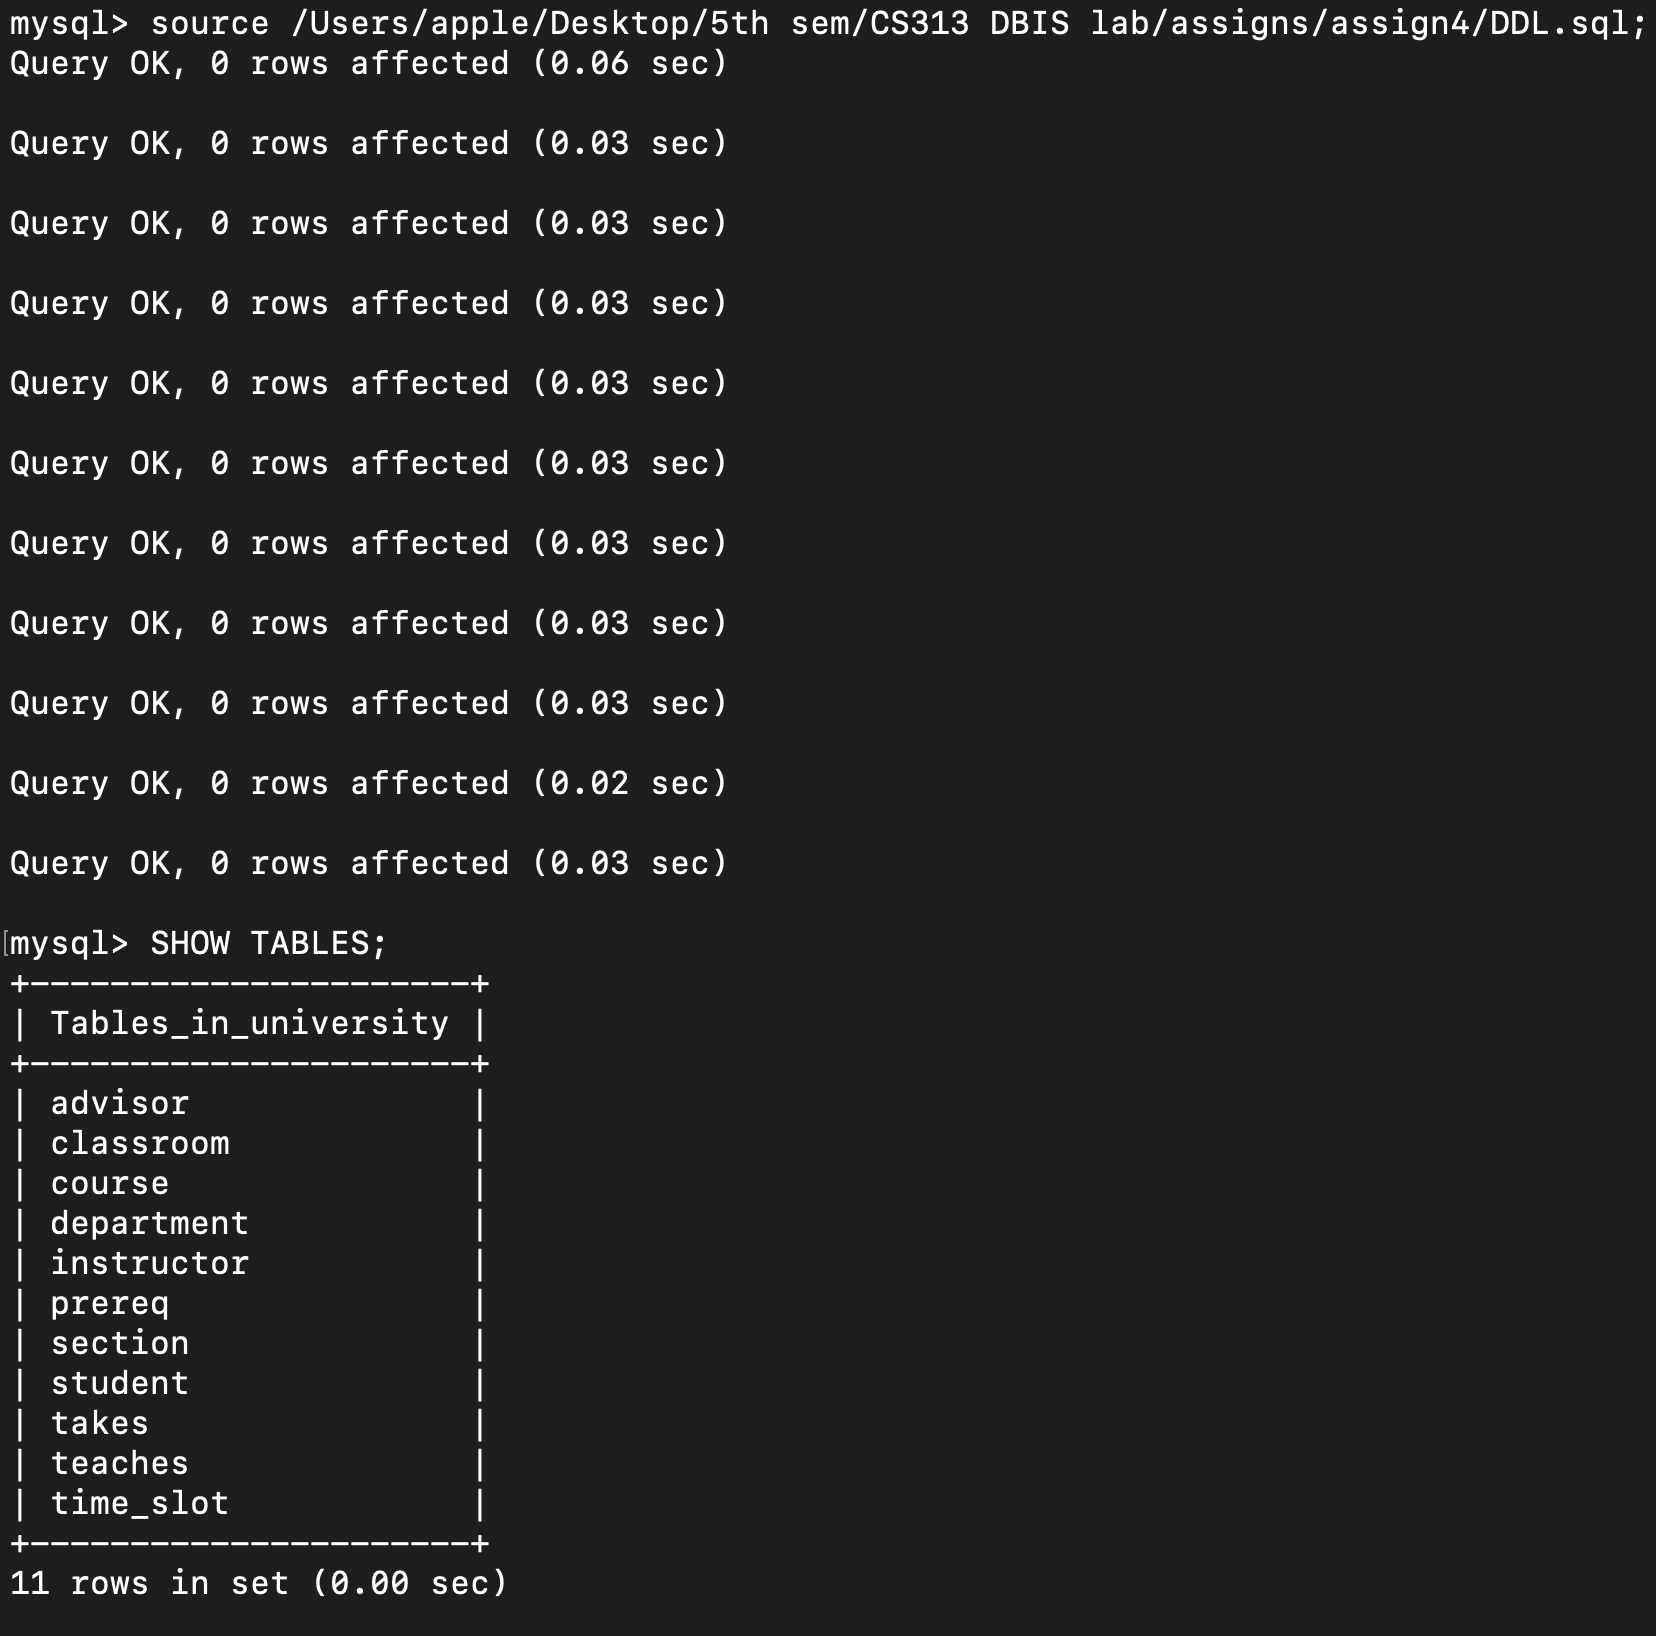
\includegraphics[scale=0.55]{screenshots/4.png}
    \label{fig:my_label1}
\end{figure}

\newpage
%---------------------------------------------------------------------
\section{Loading the data into tables using insert.sql}

\subsection{Query}
\fbox{ 
    \begin{minipage}{40em}
    \inputminted{mysql}{src/5.sql}
    \end{minipage}
}

\subsection{Result}
\begin{figure}[!hbt]
    \centering
    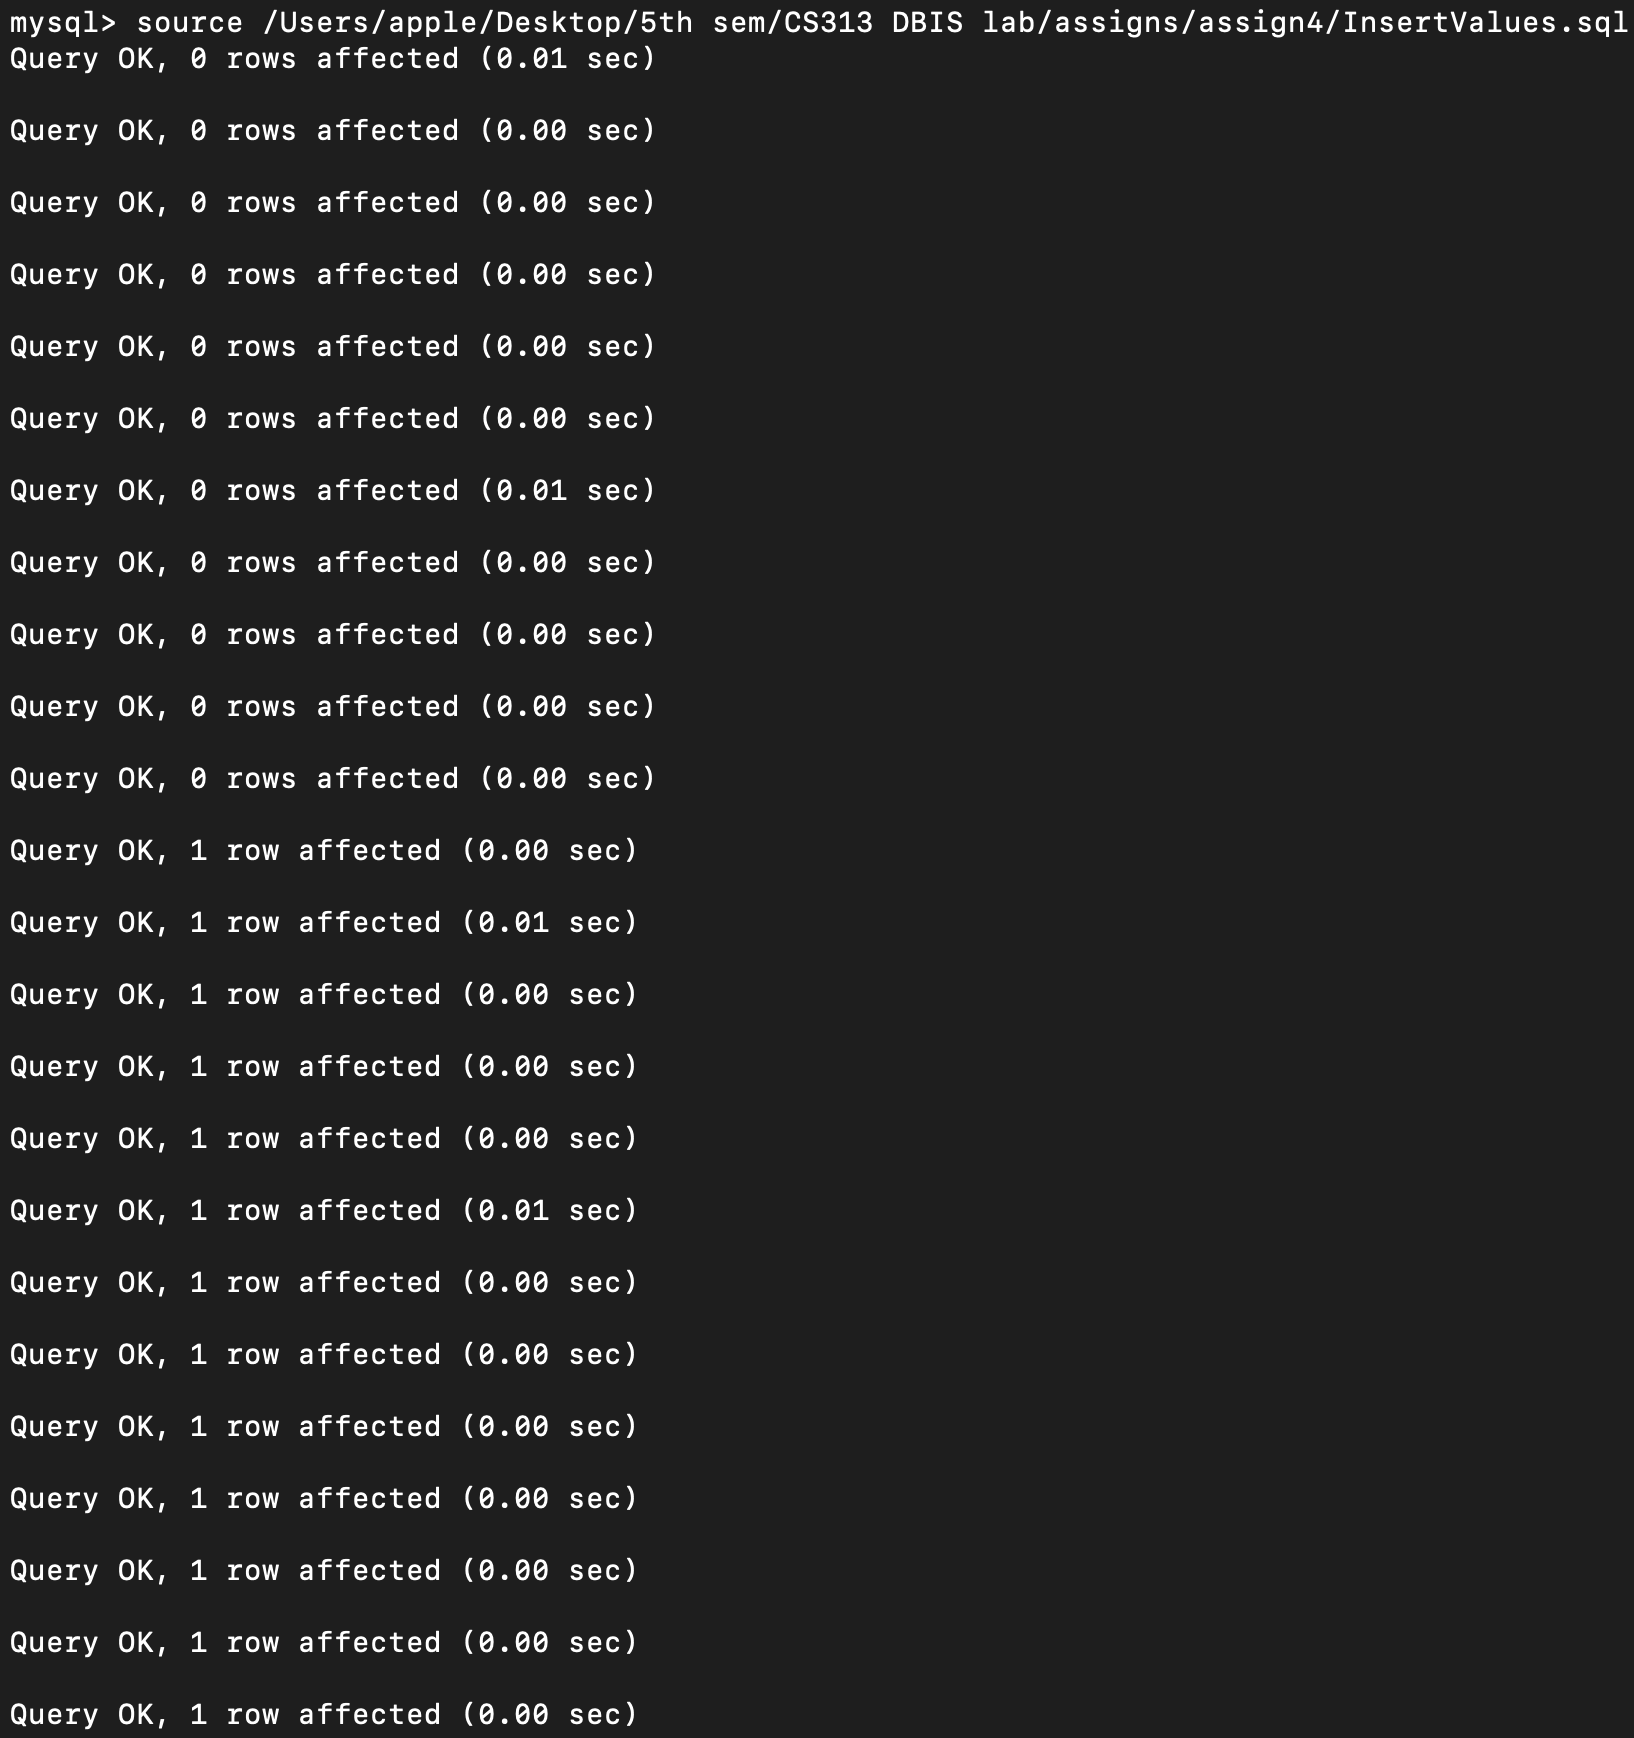
\includegraphics[scale=0.52]{screenshots/5.png}
    \label{fig:my_label1}
\end{figure}

\newpage
%---------------------------------------------------------------------

\section{Details of all the tables using information\_schema}

\subsection{Query}
\fbox{ 
    \begin{minipage}{40em}
    \inputminted{mysql}{src/6.sql}
    \end{minipage}
}

\subsection{Result}
\begin{figure}[!hbt]
    \centering
    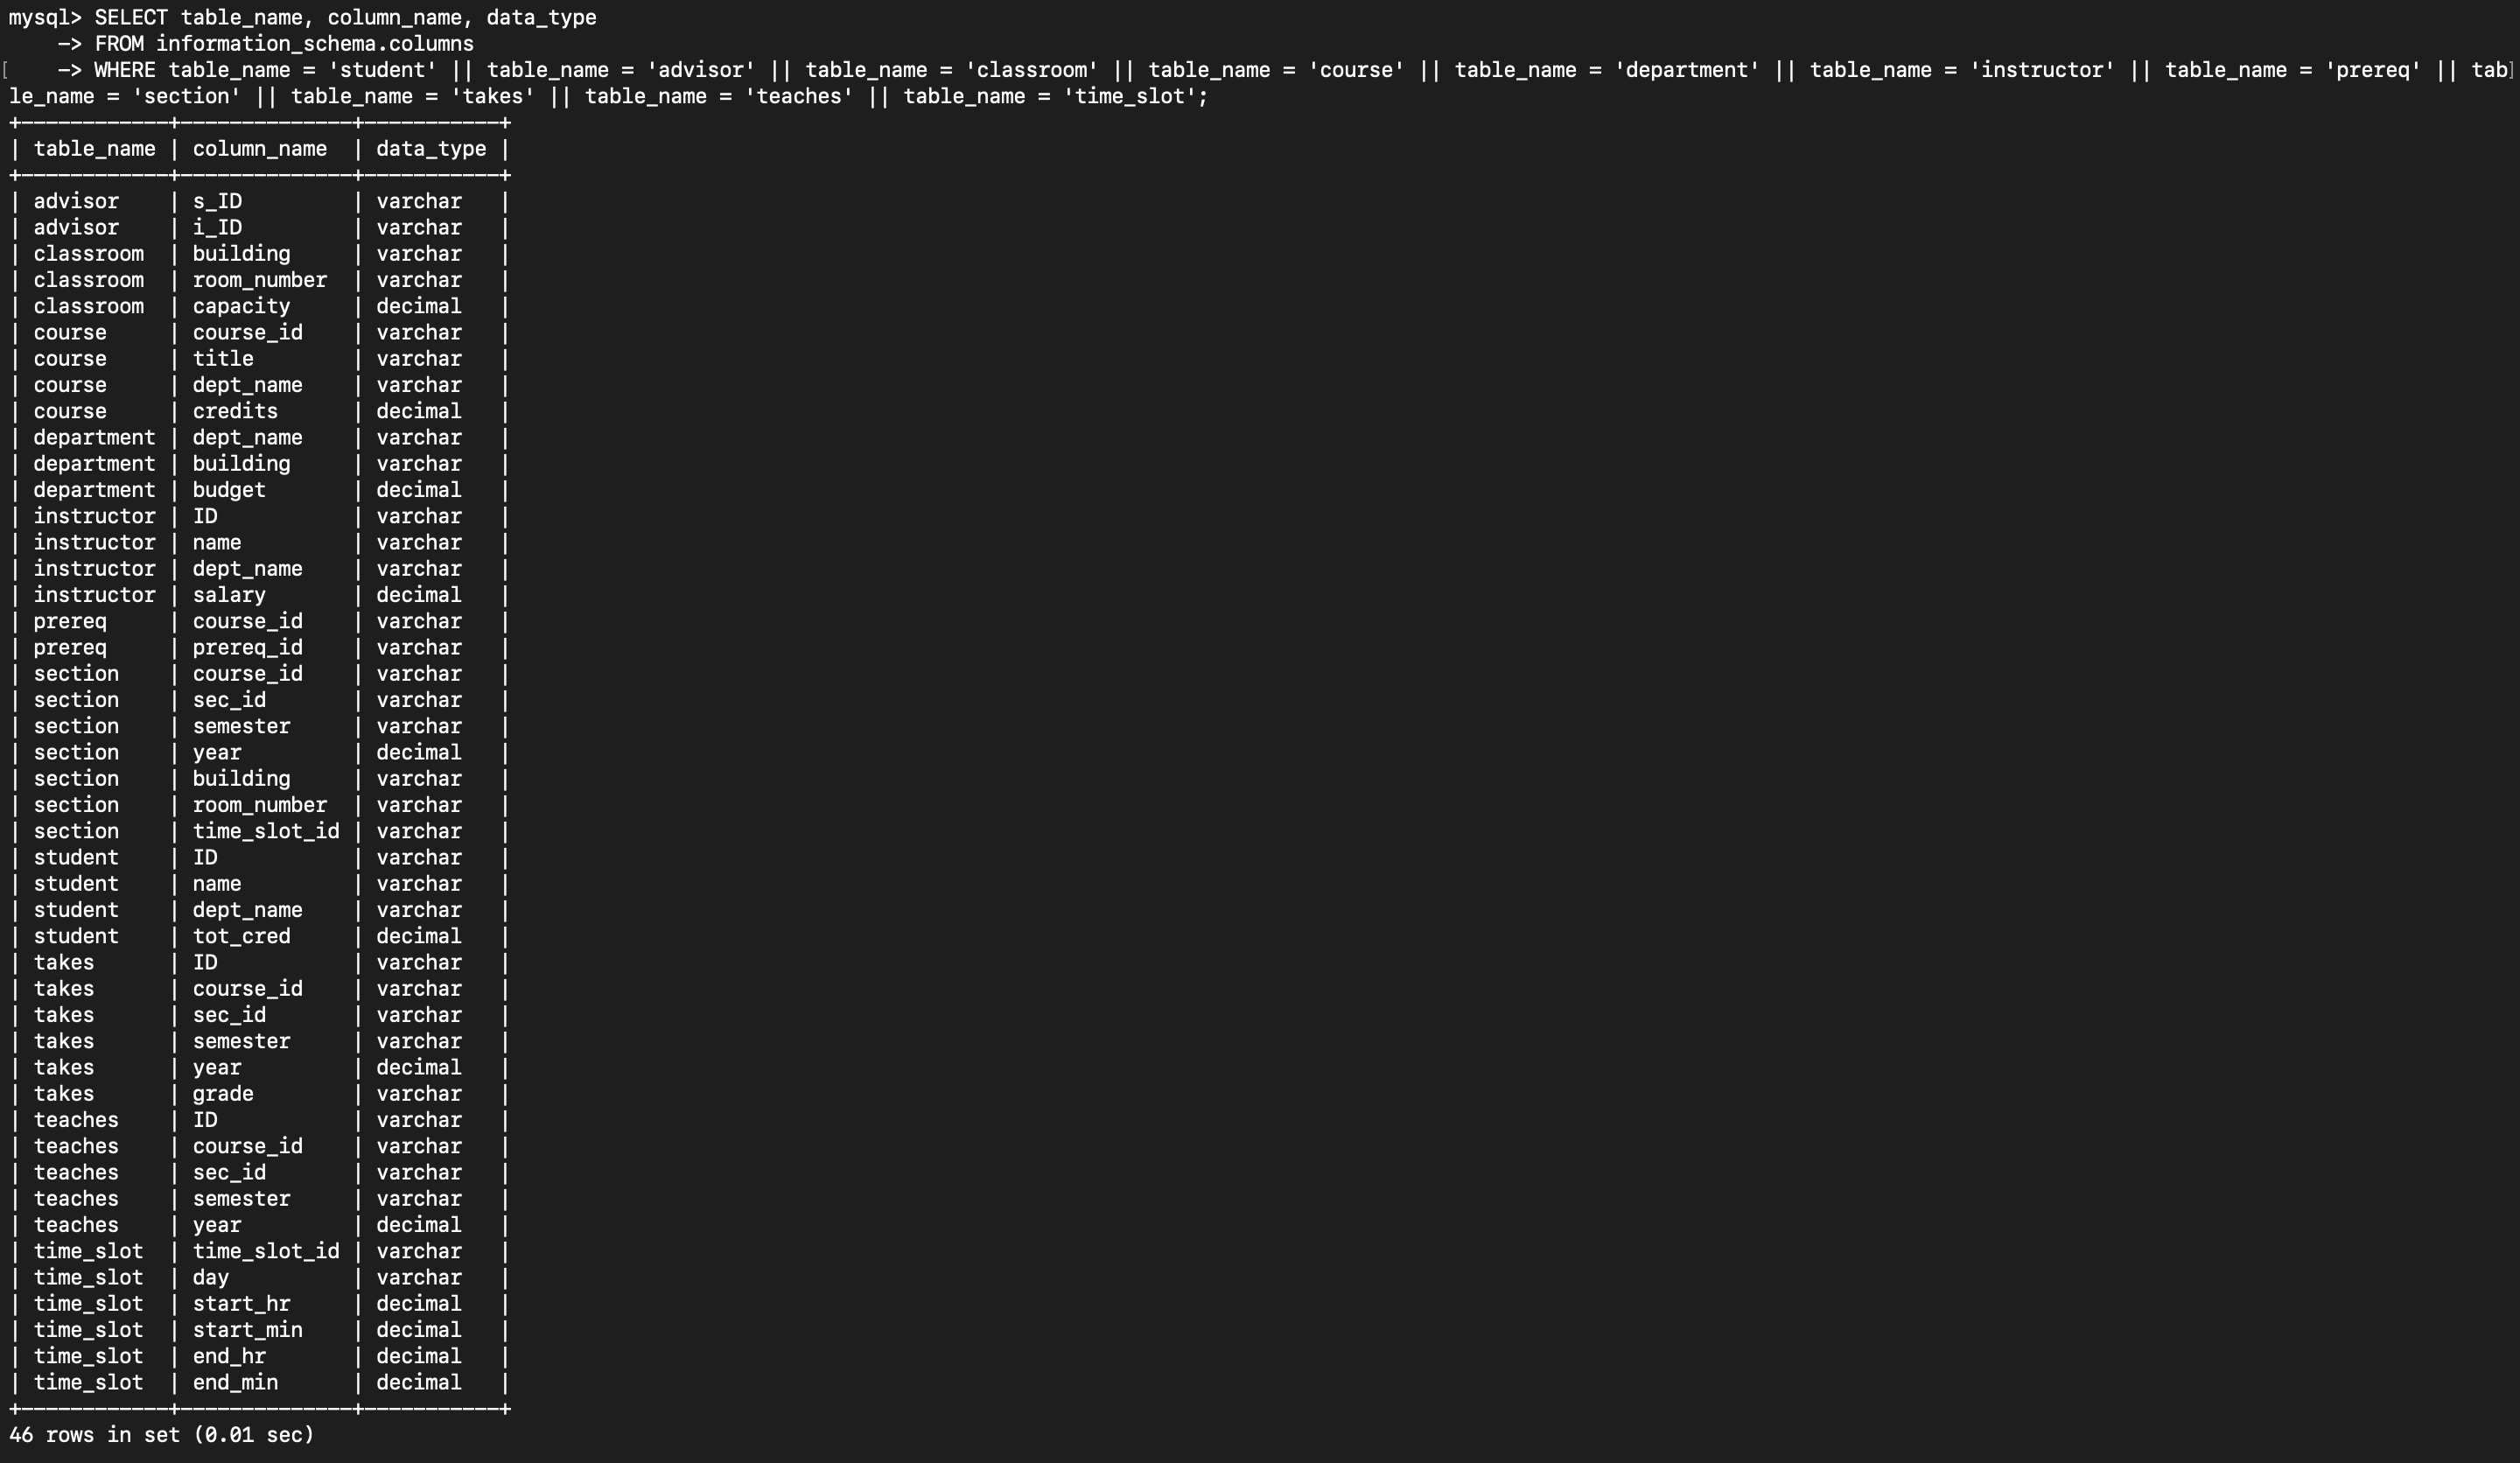
\includegraphics[scale=0.35]{screenshots/6.png}
    \label{fig:my_label1}
\end{figure}
\newpage

%---------------------------------------------------------------------

\section{Operations using \textit{phpMyAdmin} tool}

\subsection{Query}
\fbox{ 
    \begin{minipage}{40em}
    \inputminted{mysql}{src/7.sql}
    \end{minipage}
}
\newpage

\subsection{Results}

\begin{figure}[!hbt]
    \centering
    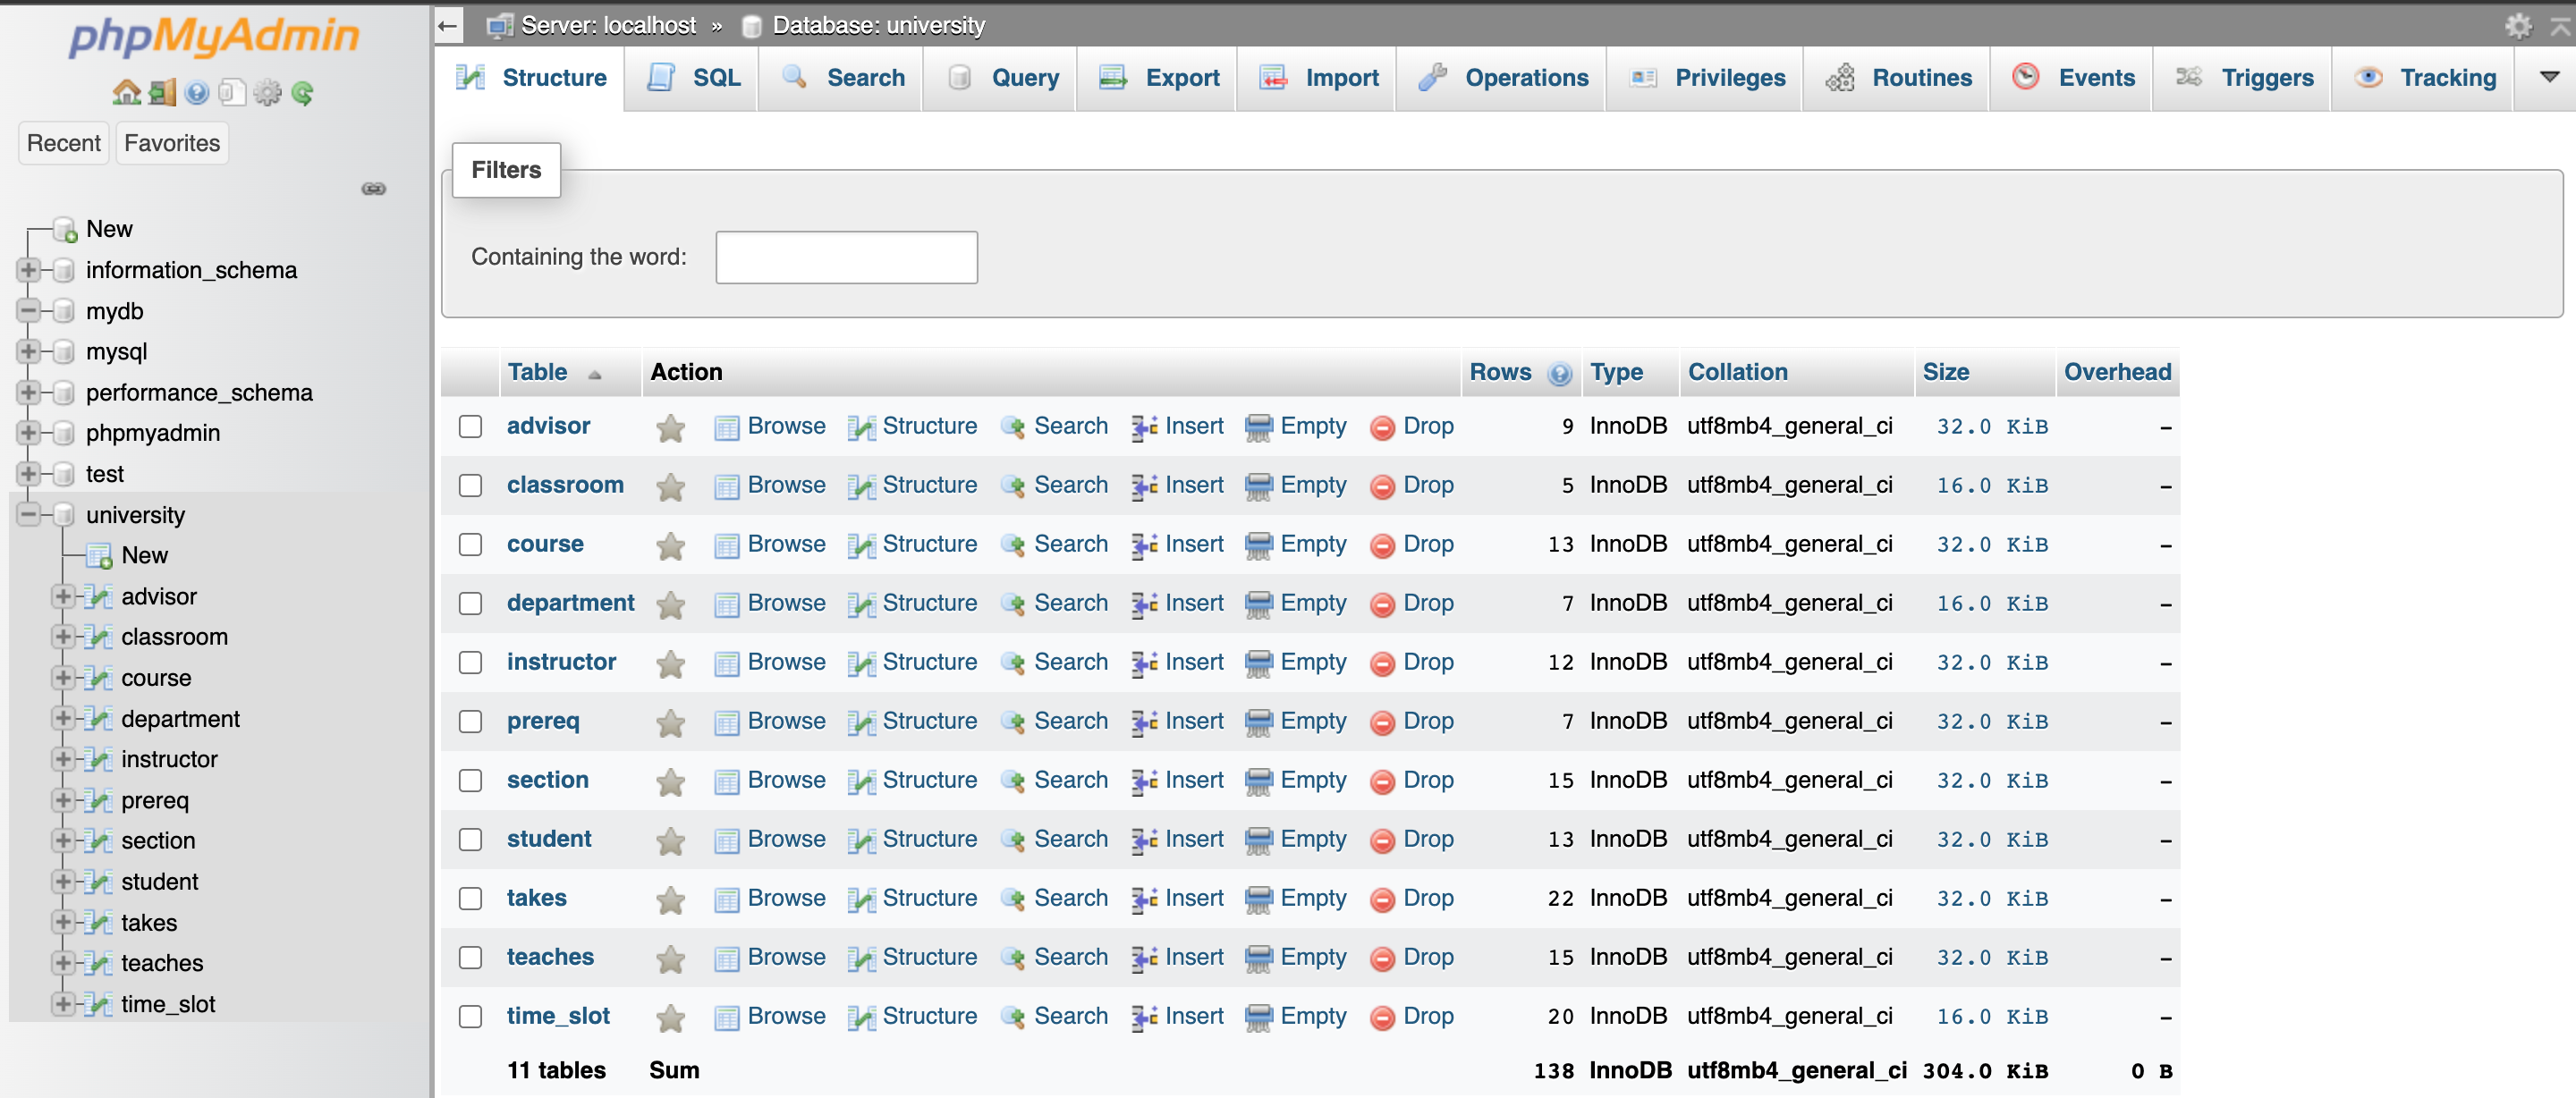
\includegraphics[scale=0.33]{screenshots/7 1.png}
    \label{fig:my_label1}
\end{figure}

\begin{figure}[!hbt]
    \centering
    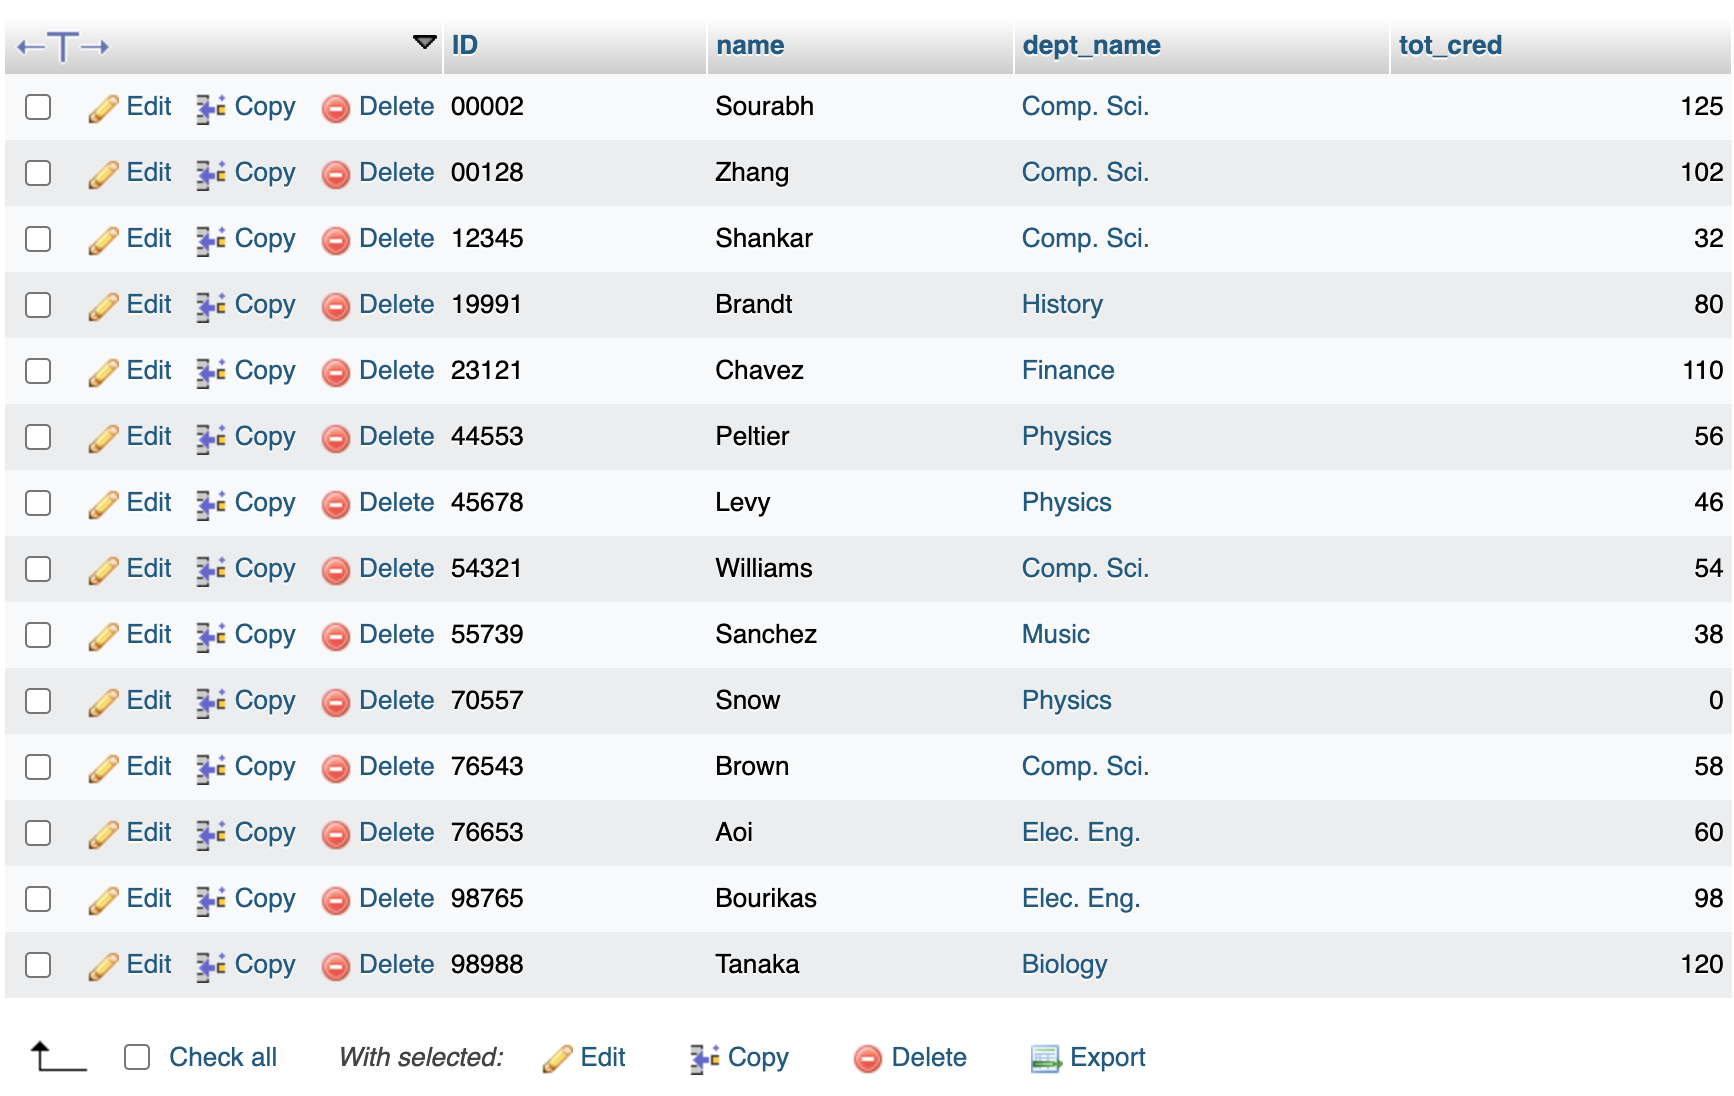
\includegraphics[scale=0.55]{screenshots/7 3 student.png}
    \label{fig:my_label1}
\end{figure}

\newpage

\begin{figure}[!hbt]
    \centering
    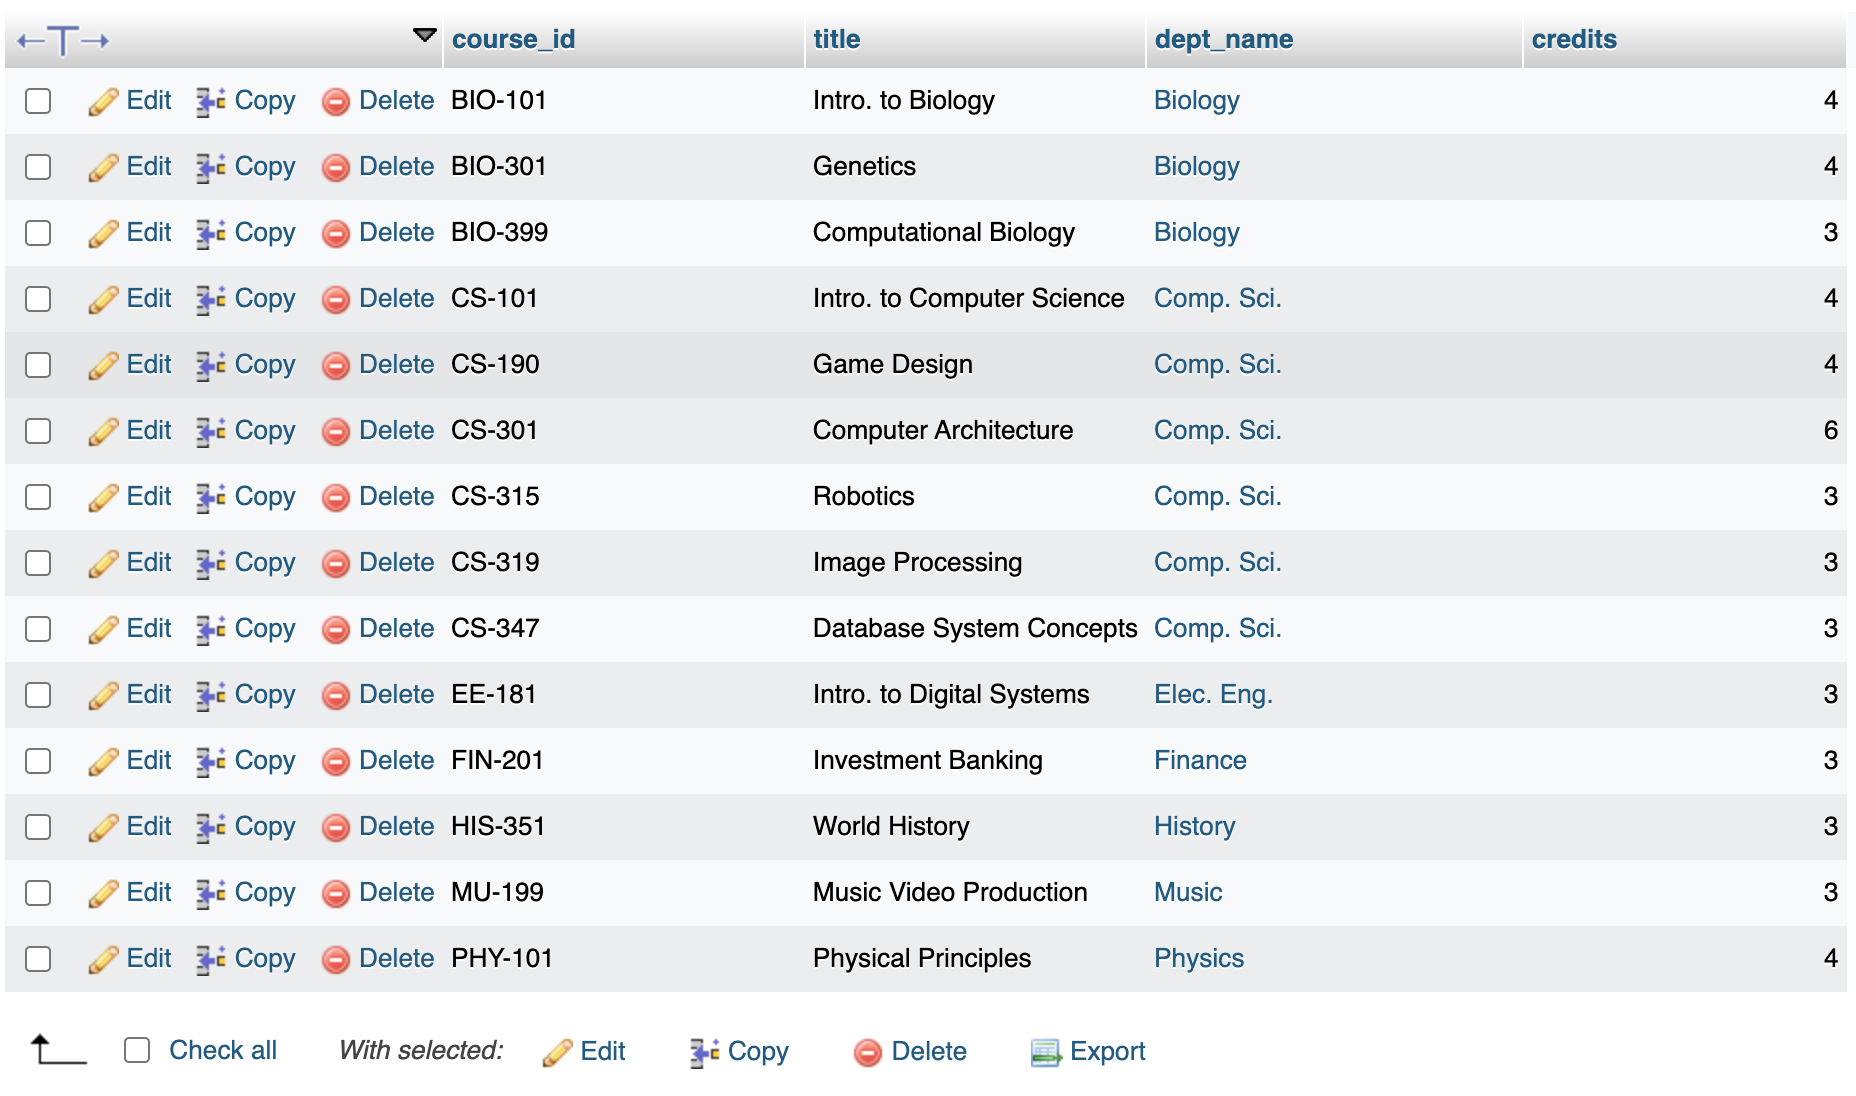
\includegraphics[scale=0.5]{screenshots/7 3 course.png}
    \label{fig:my_label1}
\end{figure}

\begin{figure}[!hbt]
    \centering
    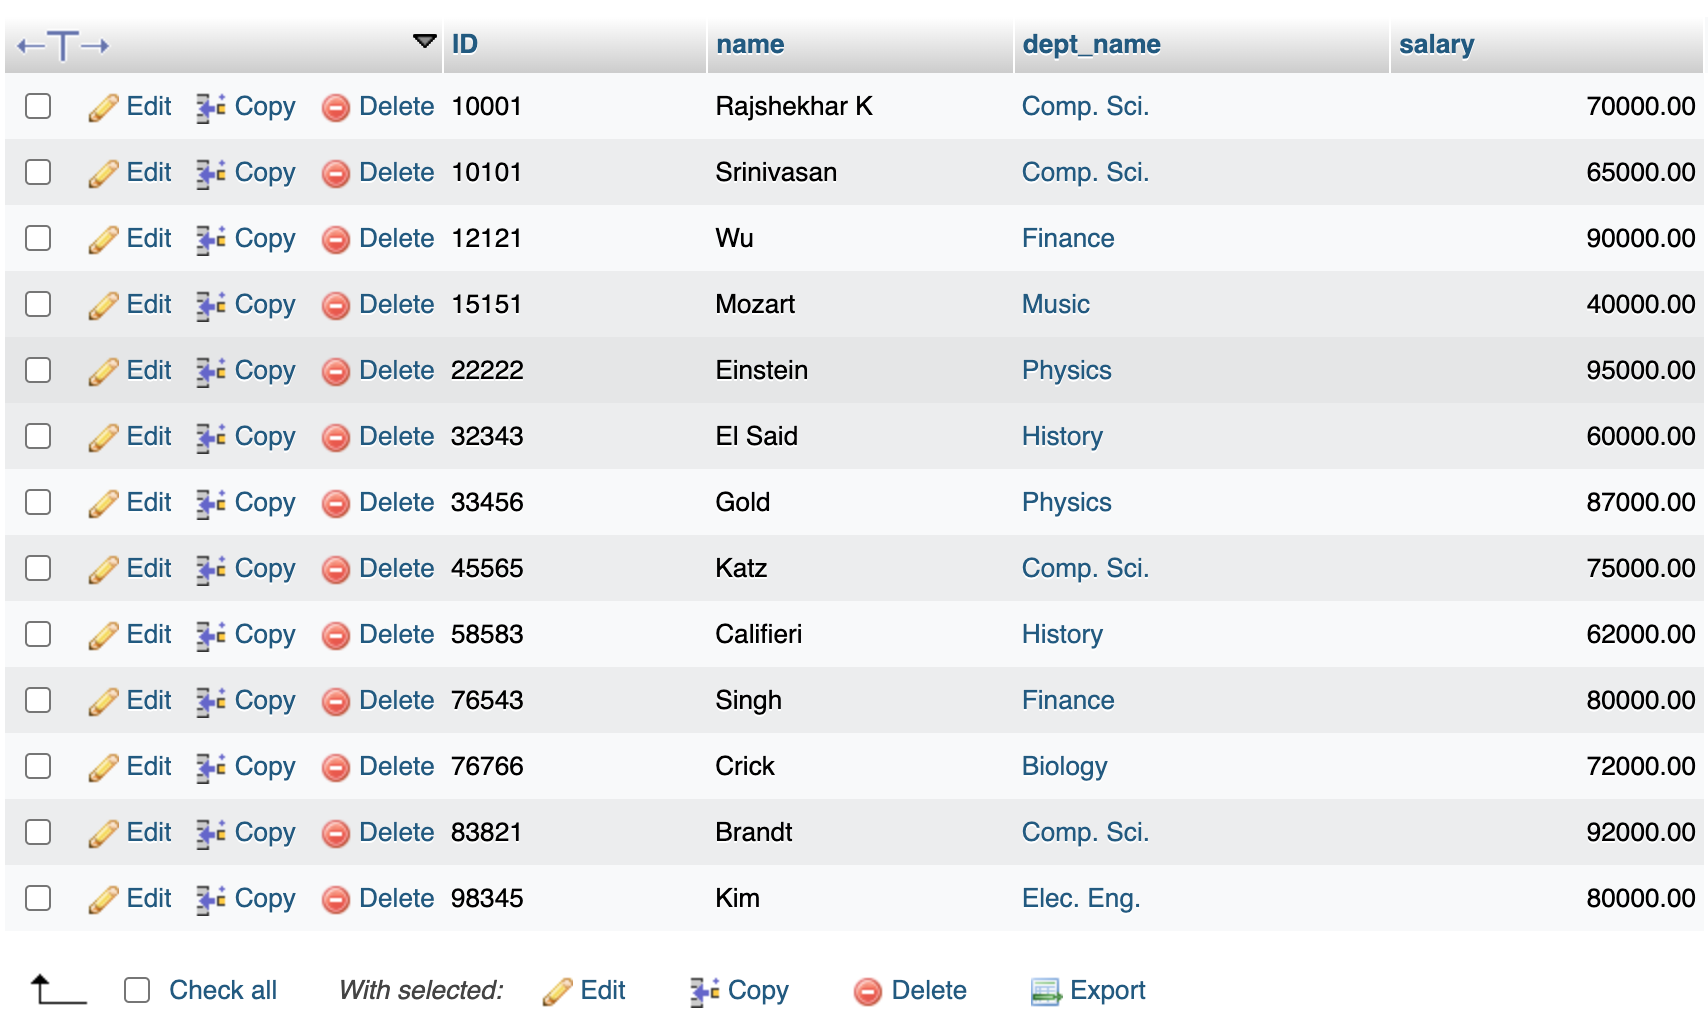
\includegraphics[scale=0.55]{screenshots/7 3 instructor.png}
    \label{fig:my_label1}
\end{figure}

\newpage

\begin{figure}[!hbt]
    \centering
    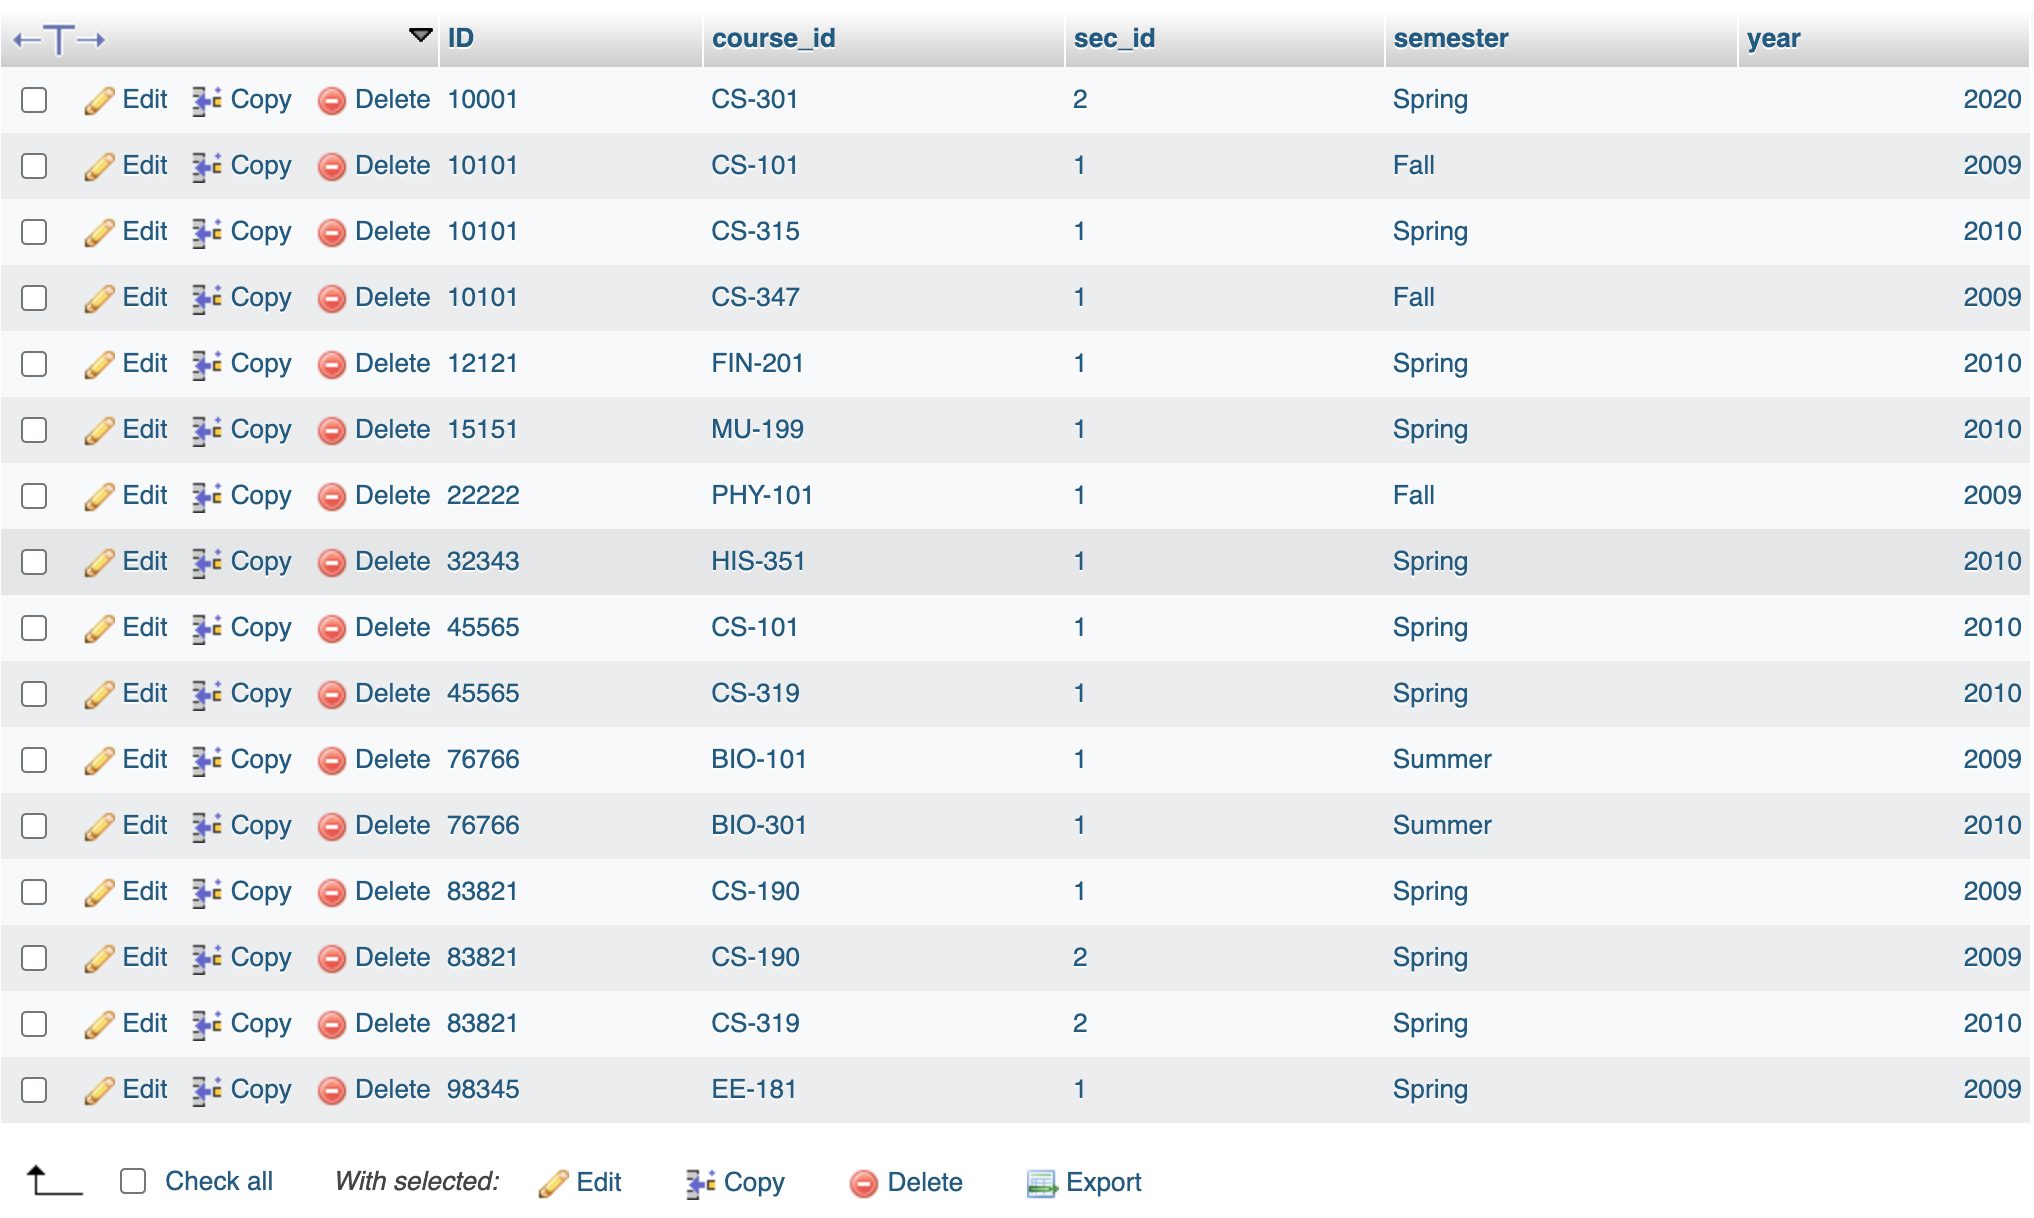
\includegraphics[scale=0.5]{screenshots/7 3 teaches.png}
    \label{fig:my_label1}
\end{figure}

\begin{figure}[!hbt]
    \centering
    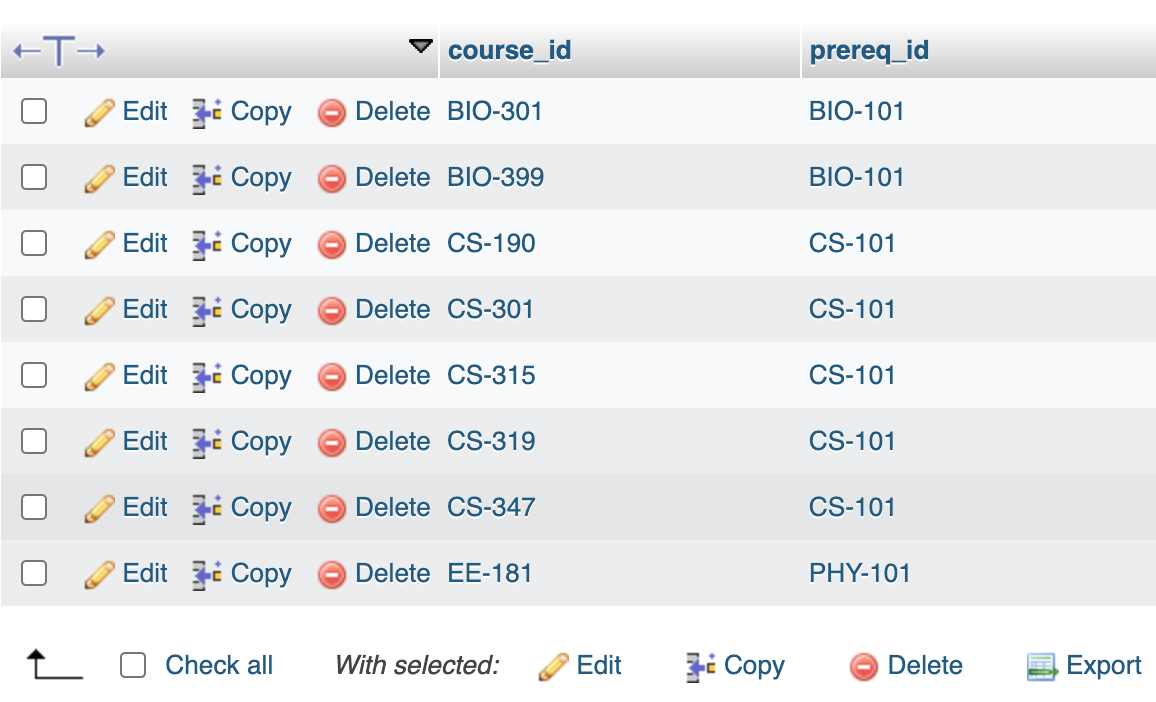
\includegraphics[scale=0.73]{screenshots/7 3 prereq.png}
    \label{fig:my_label1}
\end{figure}

\newpage

\begin{figure}[!hbt]
    \centering
    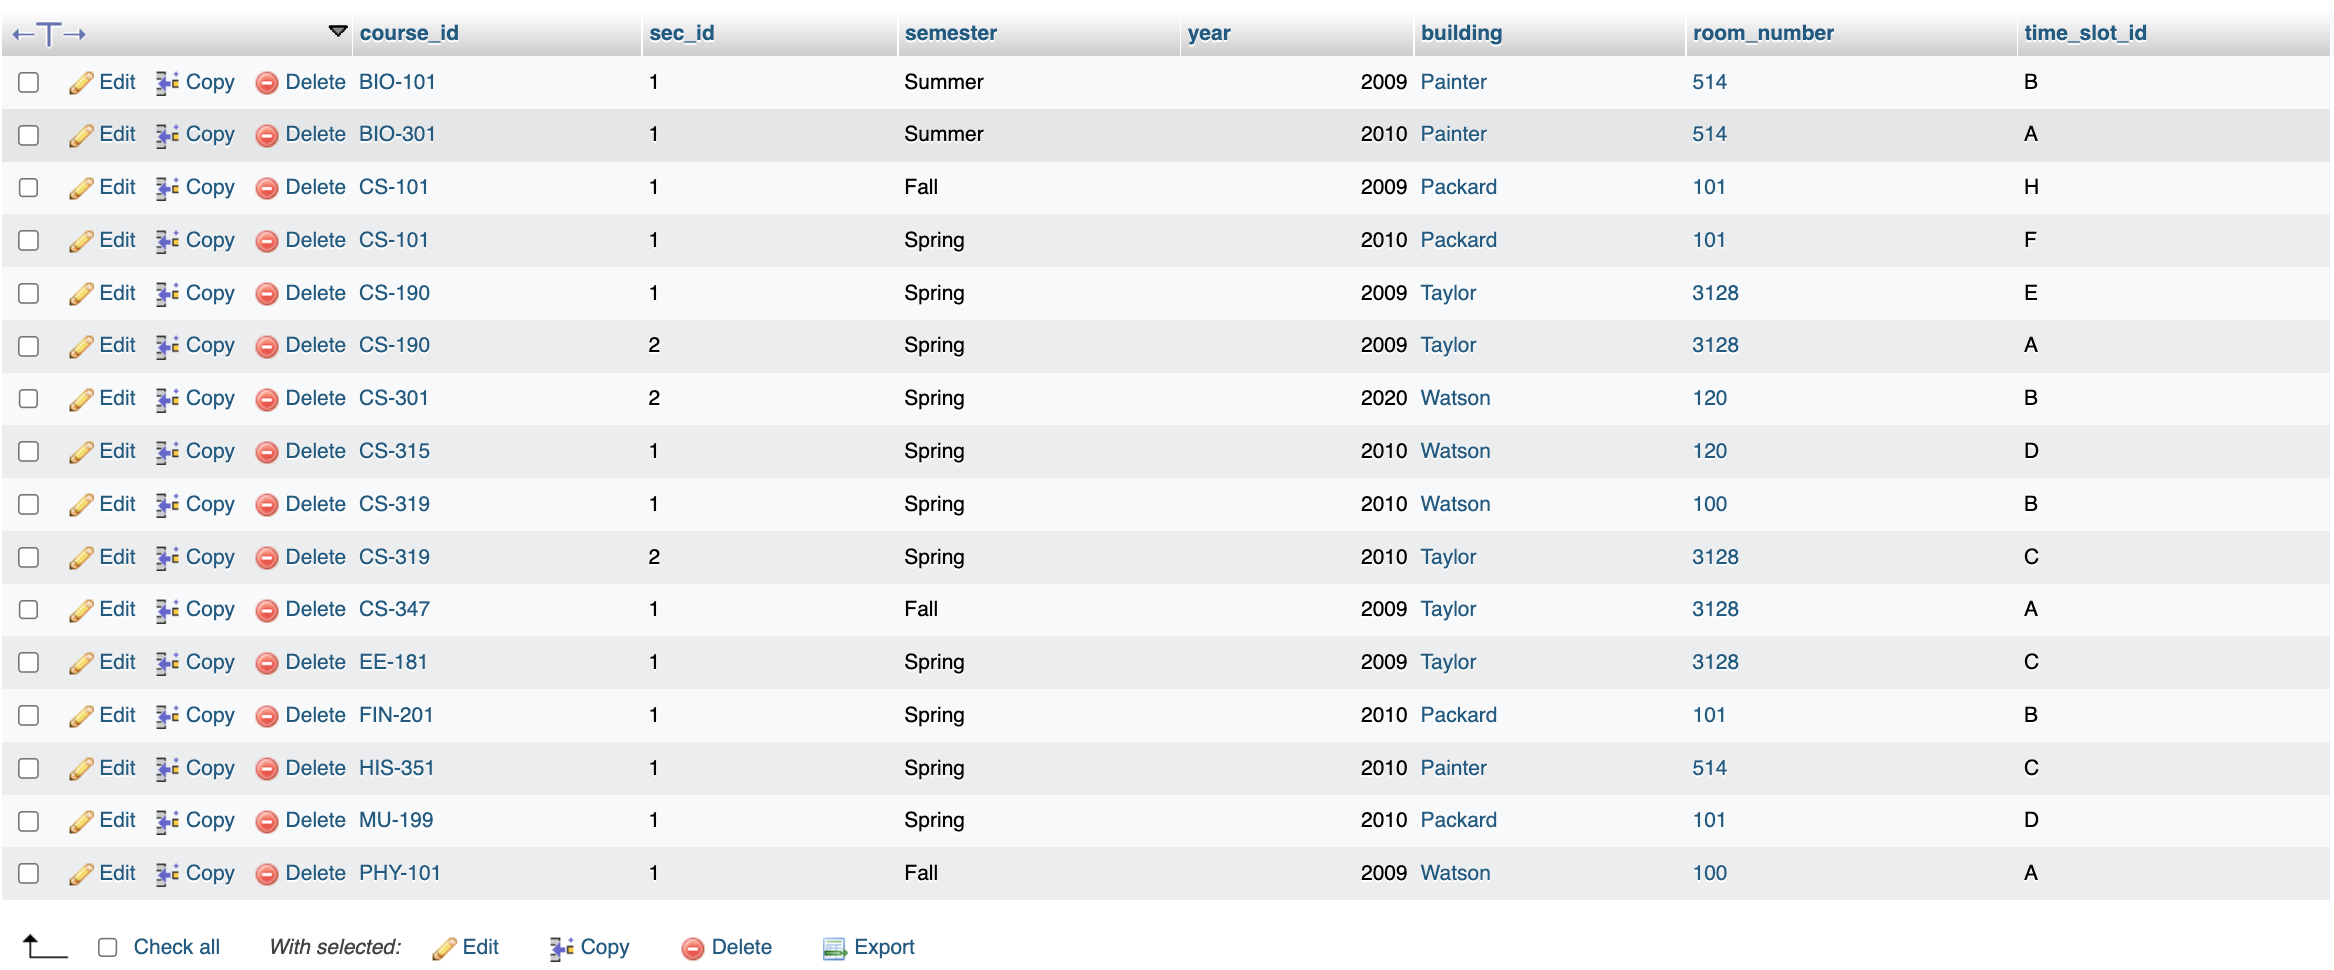
\includegraphics[scale=0.42]{screenshots/7 3 section.png}
    \label{fig:my_label1}
\end{figure}

\vspace{3cm}

\begin{figure}[!hbt]
    \centering
    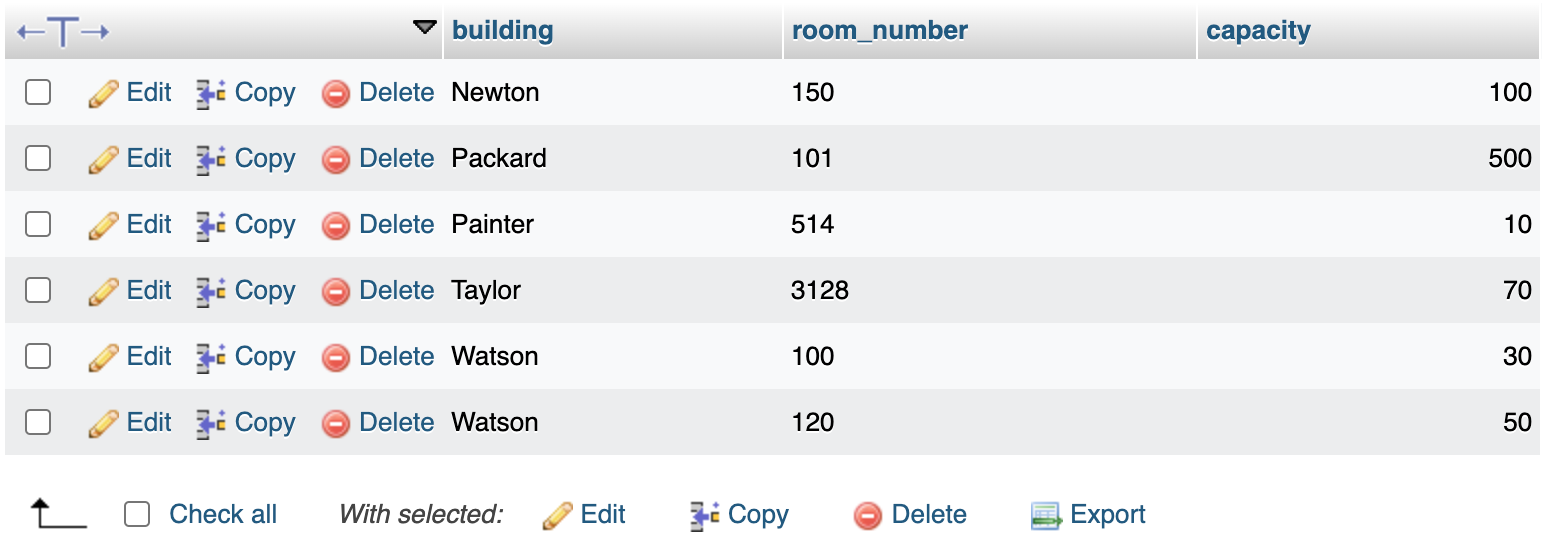
\includegraphics[scale=0.65]{screenshots/7 3 classroom.png}
    \label{fig:my_label1}
\end{figure}

\newpage

\begin{figure}[!hbt]
    \centering
    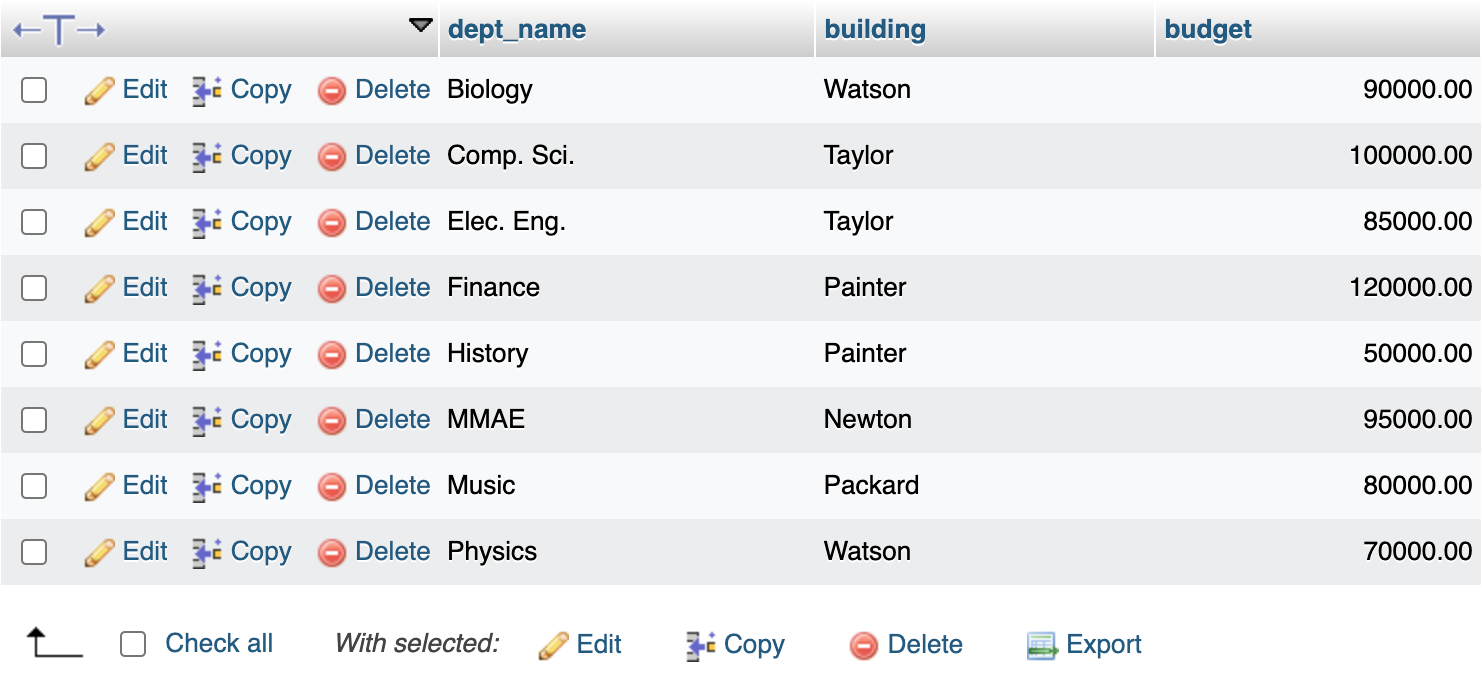
\includegraphics[scale=0.62]{screenshots/7 3 department.png}
    \label{fig:my_label1}
\end{figure}

\begin{figure}[!hbt]
    \centering
    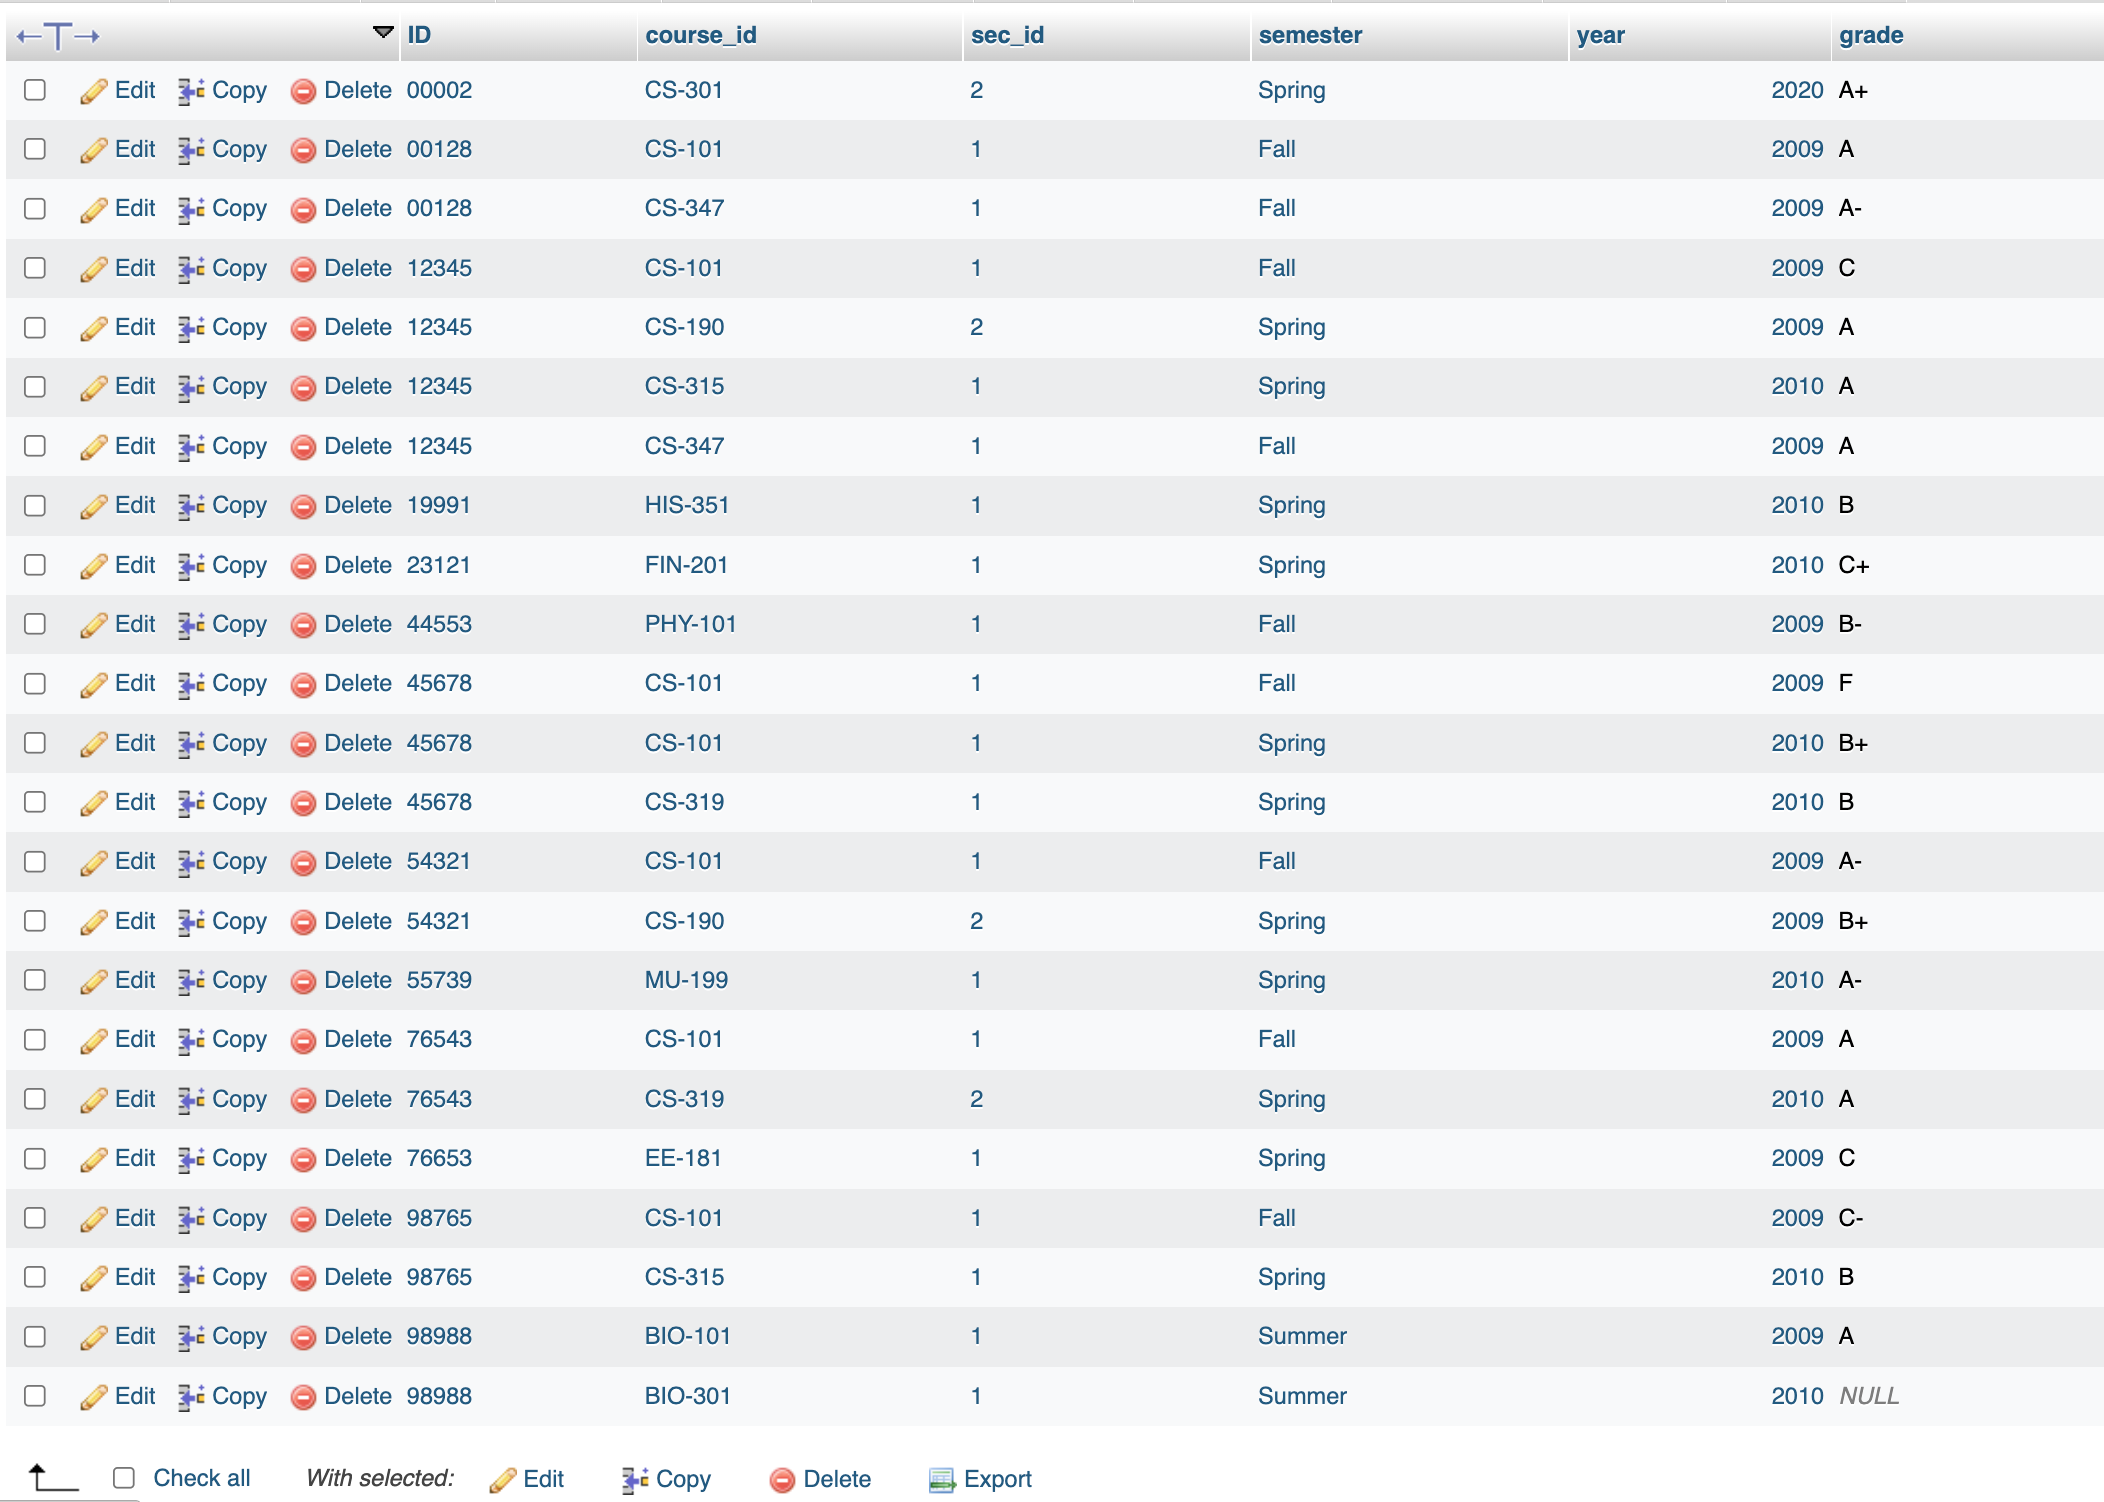
\includegraphics[scale=0.45]{screenshots/7 3 takes.png}
    \label{fig:my_label1}
\end{figure}

\newpage

\begin{figure}[!hbt]
    \centering
    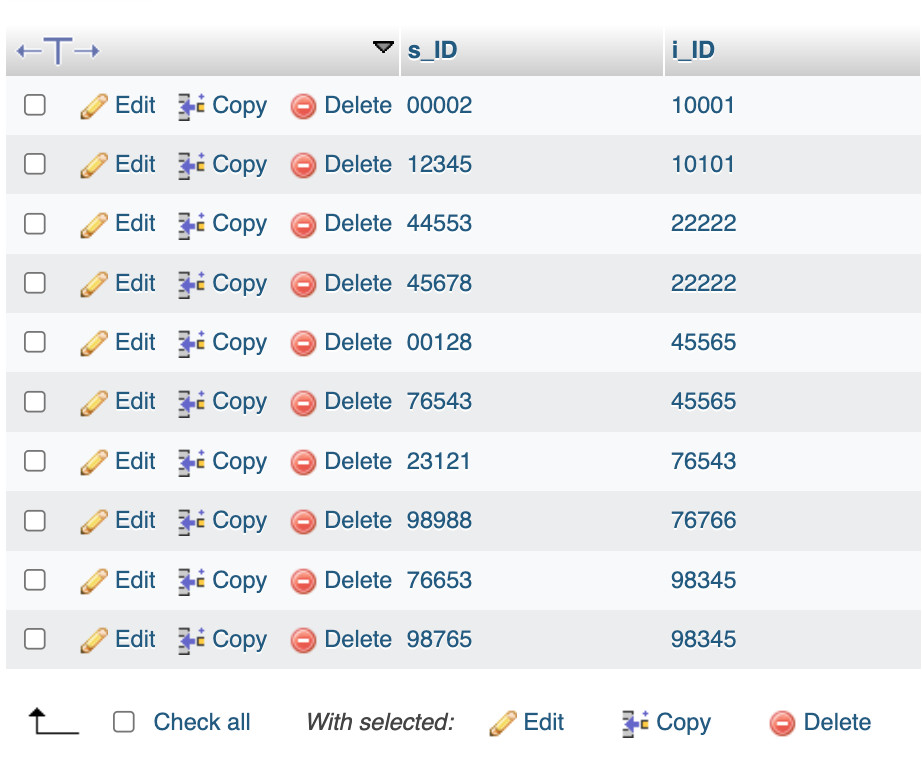
\includegraphics[scale=0.65]{screenshots/7 3 advisor.png}
    \label{fig:my_label1}
\end{figure}

\begin{figure}[!hbt]
    \centering
    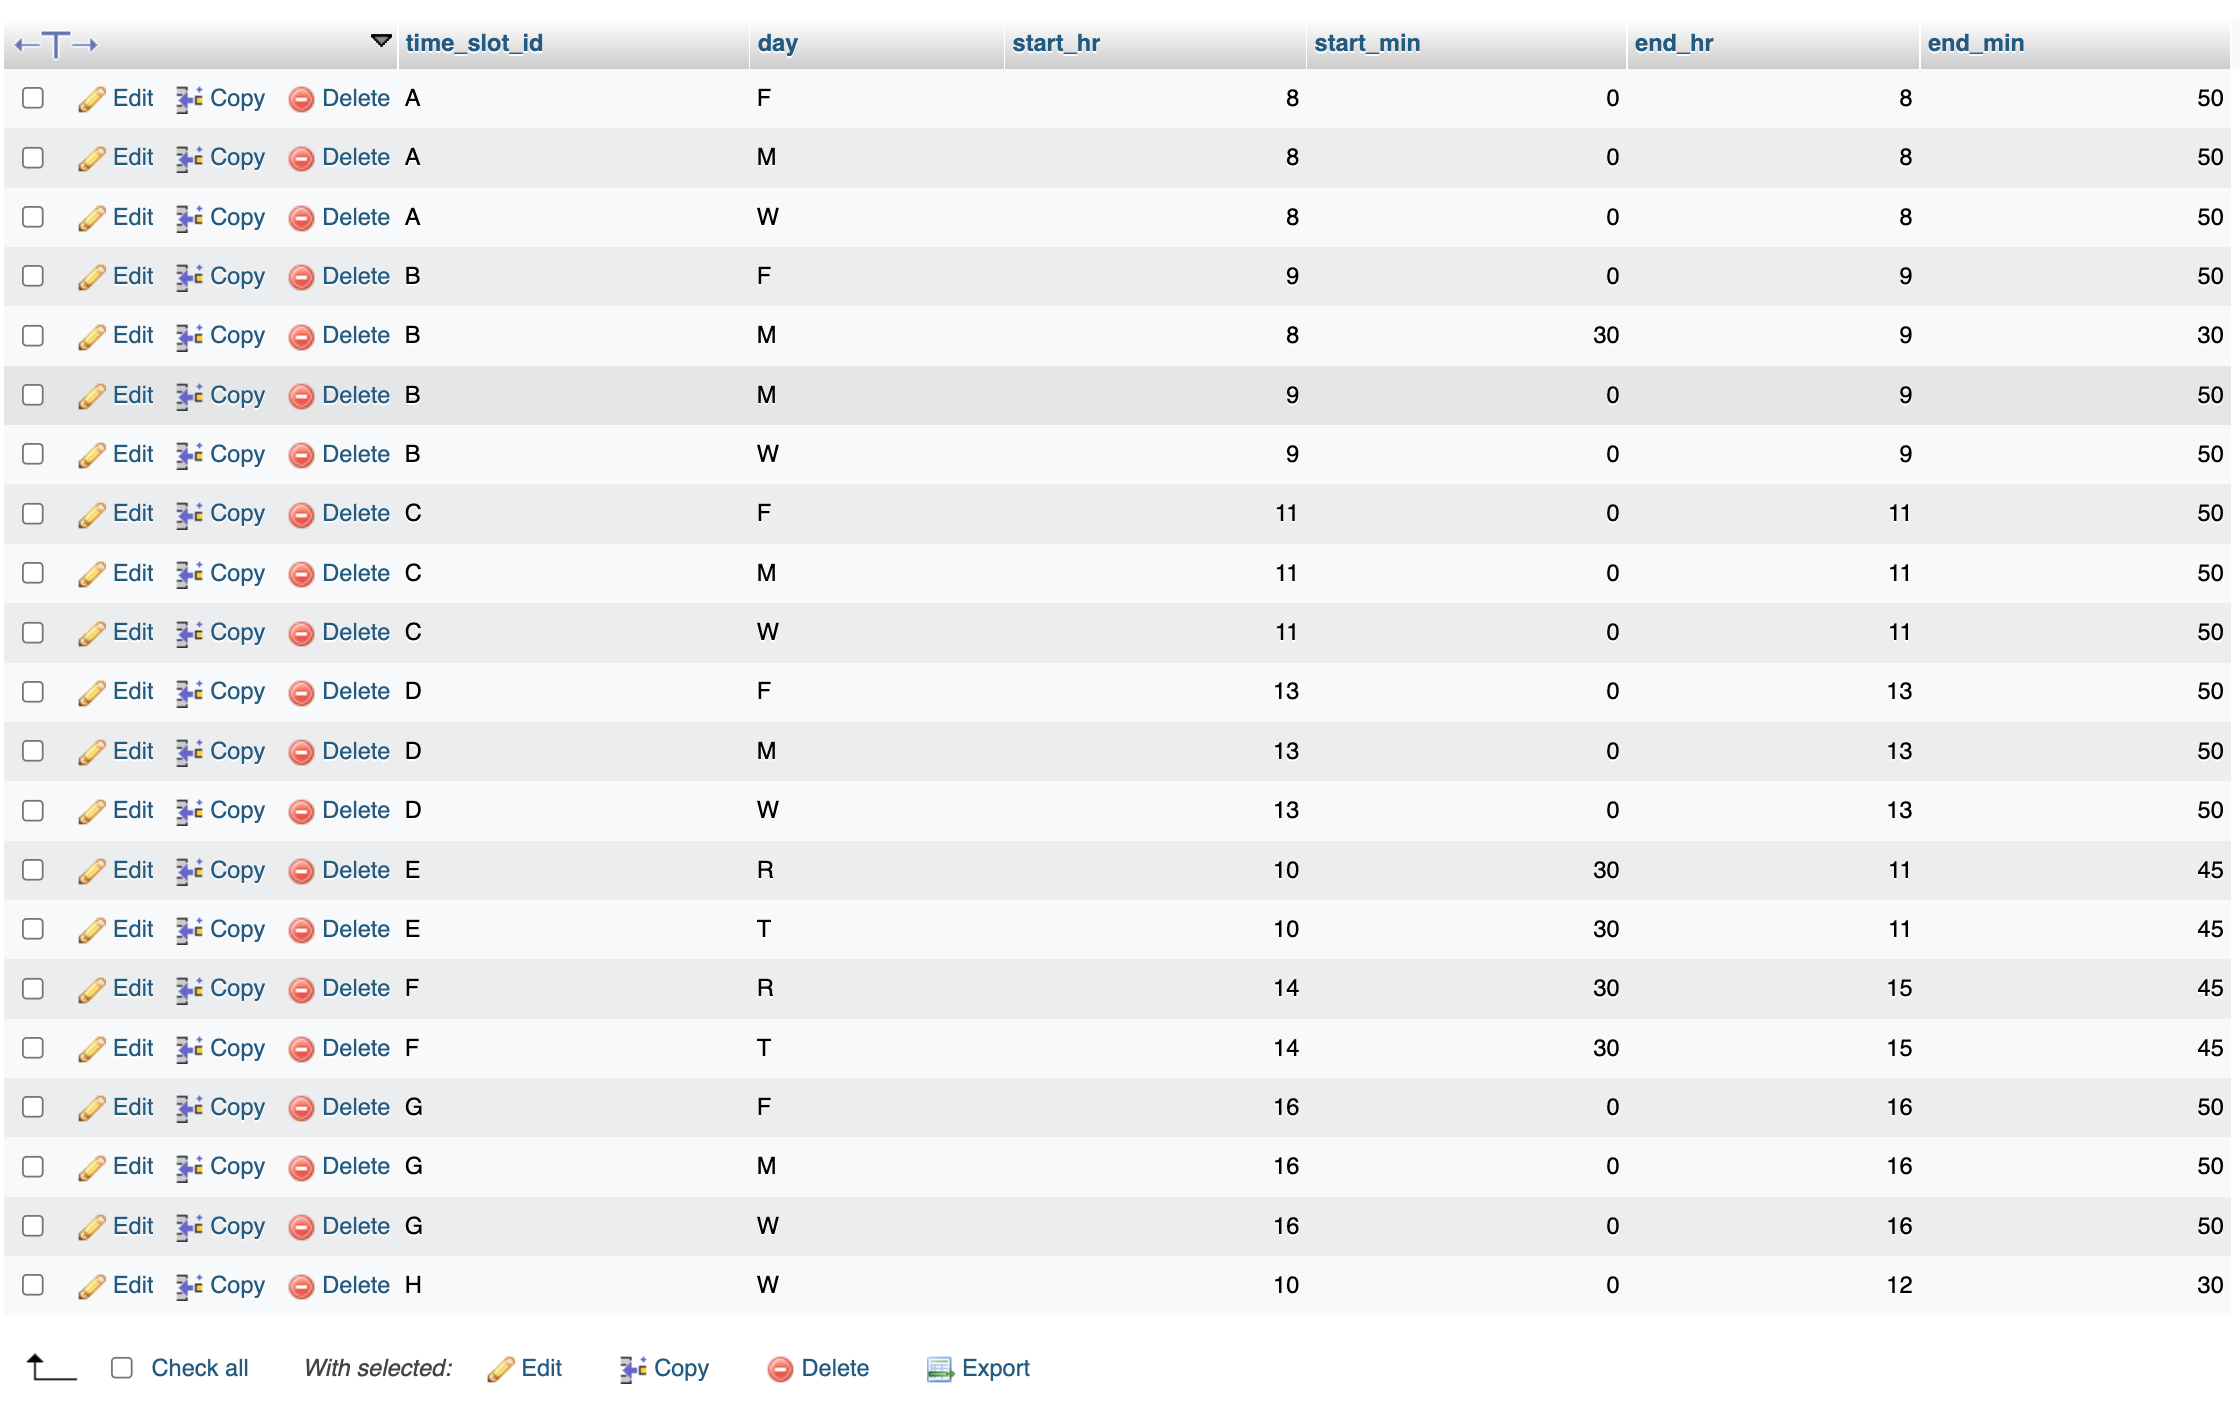
\includegraphics[scale=0.43]{screenshots/7 3 time_slot.png}
    \label{fig:my_label1}
\end{figure}

\newpage

\subsection{Inserting more data into tables for question 8}

\fbox{ 
    \begin{minipage}{40em}
    \inputminted{mysql}{src/7_8a.sql}
    \end{minipage}
}
\newpage

\fbox{ 
    \begin{minipage}{40em}
    \inputminted{mysql}{src/7_8b.sql}
    \end{minipage}
}

\newpage
%--------------------------------------------------------------
\section{SQL queries on phpMyAdmin}

\subsection{Find the course\_id, title, instructor\_id and name of those instructors who are from CSE department but are teaching a course of Civil department in the year 2009. Arrange results in ascending order of instructor names.}

\subsection*{Query}
\fbox{ 
    \begin{minipage}{40em}
    \inputminted{mysql}{src/8a.sql}
    \end{minipage}
}

\subsection*{Results}
\begin{figure}[!hbt]
    \centering
    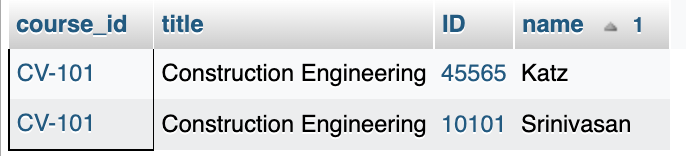
\includegraphics[scale=1.2]{screenshots/8a.png}
    \label{fig:my_label1}
\end{figure}
\newpage
%--------------------------------------------------------------

\subsection{Add a new course with course\_id as CS-333 (with suitable values for other attributes) for the CSE department which will have CS-303 as a prerequisite. Write insert statements for the same.}

\subsection*{Query}
\fbox{ 
    \begin{minipage}{40em}
    \inputminted{mysql}{src/8b.sql}
    \end{minipage}
}

\subsection*{Results}
\begin{figure}[!hbt]
    \centering
    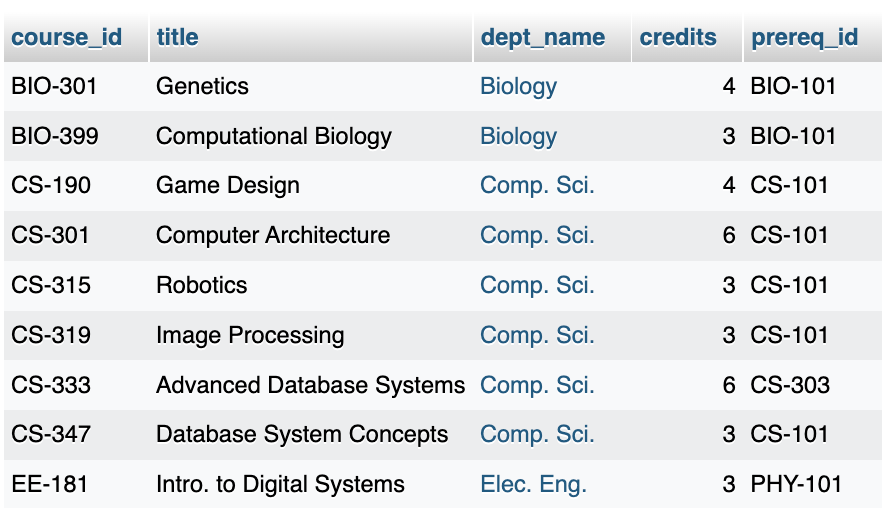
\includegraphics[scale=1.1]{screenshots/8b.png}
    \label{fig:my_label1}
\end{figure}
\newpage
%--------------------------------------------------------------

\subsection{Update salaries of instructors by 10\% if their departments have a budget of more than 900000 rupees. Write the update statements for the same.}

\subsection*{Query}
\fbox{ 
    \begin{minipage}{40em}
    \inputminted{mysql}{src/8c.sql}
    \end{minipage}
}

\subsection*{Results}
\begin{figure}[!hbt]
    \centering
    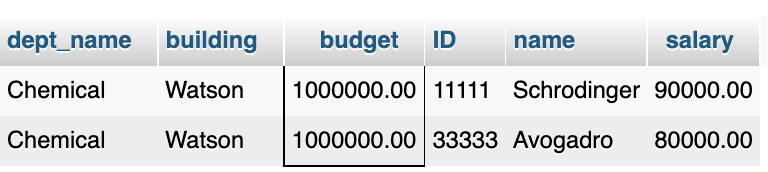
\includegraphics[scale=1.1]{screenshots/8c 1.png}
    \label{fig:my_label1}
    \caption{Table before updation}
\end{figure}

\begin{figure}[!hbt]
    \centering
    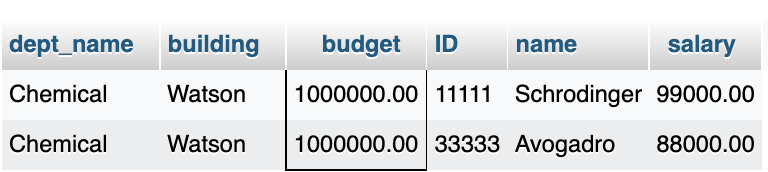
\includegraphics[scale=1.1]{screenshots/8c 2.png}
    \label{fig:my_label1}
    \caption{Table after updation}
\end{figure}
\newpage
%--------------------------------------------------------------

\subsection{Find CSE department courses (id and title) and number of students taking that course in the year 2007 and semester Fall where the number is greater than 15. Arrange the results in ascending order of course id.}

\subsection*{Query}
\fbox{ 
    \begin{minipage}{40em}
    \inputminted{mysql}{src/8d.sql}
    \end{minipage}
}

\subsection*{Results}
\begin{figure}[!hbt]
    \centering
    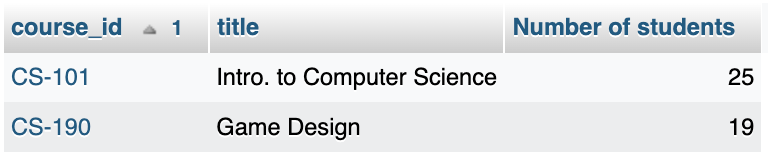
\includegraphics[scale=1.2]{screenshots/8d.png}
    \label{fig:my_label1}
\end{figure}
%--------------------------------------------------------------

\end{document}